\documentclass[1p]{elsarticle_modified}
%\bibliographystyle{elsarticle-num}

%\usepackage[colorlinks]{hyperref}
%\usepackage{abbrmath_seonhwa} %\Abb, \Ascr, \Acal ,\Abf, \Afrak
\usepackage{amsfonts}
\usepackage{amssymb}
\usepackage{amsmath}
\usepackage{amsthm}
\usepackage{scalefnt}
\usepackage{amsbsy}
\usepackage{kotex}
\usepackage{caption}
\usepackage{subfig}
\usepackage{color}
\usepackage{graphicx}
\usepackage{xcolor} %% white, black, red, green, blue, cyan, magenta, yellow
\usepackage{float}
\usepackage{setspace}
\usepackage{hyperref}

\usepackage{tikz}
\usetikzlibrary{arrows}

\usepackage{multirow}
\usepackage{array} % fixed length table
\usepackage{hhline}

%%%%%%%%%%%%%%%%%%%%%
\makeatletter
\renewcommand*\env@matrix[1][\arraystretch]{%
	\edef\arraystretch{#1}%
	\hskip -\arraycolsep
	\let\@ifnextchar\new@ifnextchar
	\array{*\c@MaxMatrixCols c}}
\makeatother %https://tex.stackexchange.com/questions/14071/how-can-i-increase-the-line-spacing-in-a-matrix
%%%%%%%%%%%%%%%

\usepackage[normalem]{ulem}

\newcommand{\msout}[1]{\ifmmode\text{\sout{\ensuremath{#1}}}\else\sout{#1}\fi}
%SOURCE: \msout is \stkout macro in https://tex.stackexchange.com/questions/20609/strikeout-in-math-mode

\newcommand{\cancel}[1]{
	\ifmmode
	{\color{red}\msout{#1}}
	\else
	{\color{red}\sout{#1}}
	\fi
}

\newcommand{\add}[1]{
	{\color{blue}\uwave{#1}}
}

\newcommand{\replace}[2]{
	\ifmmode
	{\color{red}\msout{#1}}{\color{blue}\uwave{#2}}
	\else
	{\color{red}\sout{#1}}{\color{blue}\uwave{#2}}
	\fi
}

\newcommand{\Sol}{\mathcal{S}} %segment
\newcommand{\D}{D} %diagram
\newcommand{\A}{\mathcal{A}} %arc


%%%%%%%%%%%%%%%%%%%%%%%%%%%%%5 test

\def\sl{\operatorname{\textup{SL}}(2,\Cbb)}
\def\psl{\operatorname{\textup{PSL}}(2,\Cbb)}
\def\quan{\mkern 1mu \triangleright \mkern 1mu}

\theoremstyle{definition}
\newtheorem{thm}{Theorem}[section]
\newtheorem{prop}[thm]{Proposition}
\newtheorem{lem}[thm]{Lemma}
\newtheorem{ques}[thm]{Question}
\newtheorem{cor}[thm]{Corollary}
\newtheorem{defn}[thm]{Definition}
\newtheorem{exam}[thm]{Example}
\newtheorem{rmk}[thm]{Remark}
\newtheorem{alg}[thm]{Algorithm}

\newcommand{\I}{\sqrt{-1}}
\begin{document}

%\begin{frontmatter}
%
%\title{Boundary parabolic representations of knots up to 8 crossings}
%
%%% Group authors per affiliation:
%\author{Yunhi Cho} 
%\address{Department of Mathematics, University of Seoul, Seoul, Korea}
%\ead{yhcho@uos.ac.kr}
%
%
%\author{Seonhwa Kim} %\fnref{s_kim}}
%\address{Center for Geometry and Physics, Institute for Basic Science, Pohang, 37673, Korea}
%\ead{ryeona17@ibs.re.kr}
%
%\author{Hyuk Kim}
%\address{Department of Mathematical Sciences, Seoul National University, Seoul 08826, Korea}
%\ead{hyukkim@snu.ac.kr}
%
%\author{Seokbeom Yoon}
%\address{Department of Mathematical Sciences, Seoul National University, Seoul, 08826,  Korea}
%\ead{sbyoon15@snu.ac.kr}
%
%\begin{abstract}
%We find all boundary parabolic representation of knots up to 8 crossings.
%
%\end{abstract}
%\begin{keyword}
%    \MSC[2010] 57M25 
%\end{keyword}
%
%\end{frontmatter}

%\linenumbers
%\tableofcontents
%
\newcommand\colored[1]{\textcolor{white}{\rule[-0.35ex]{0.8em}{1.4ex}}\kern-0.8em\color{red} #1}%
%\newcommand\colored[1]{\textcolor{white}{ #1}\kern-2.17ex	\textcolor{white}{ #1}\kern-1.81ex	\textcolor{white}{ #1}\kern-2.15ex\color{red}#1	}

{\Large $\underline{12a_{0958}~(K12a_{0958})}$}

\setlength{\tabcolsep}{10pt}
\renewcommand{\arraystretch}{1.6}
\vspace{1cm}\begin{tabular}{m{100pt}>{\centering\arraybackslash}m{274pt}}
\multirow{5}{120pt}{
	\centering
	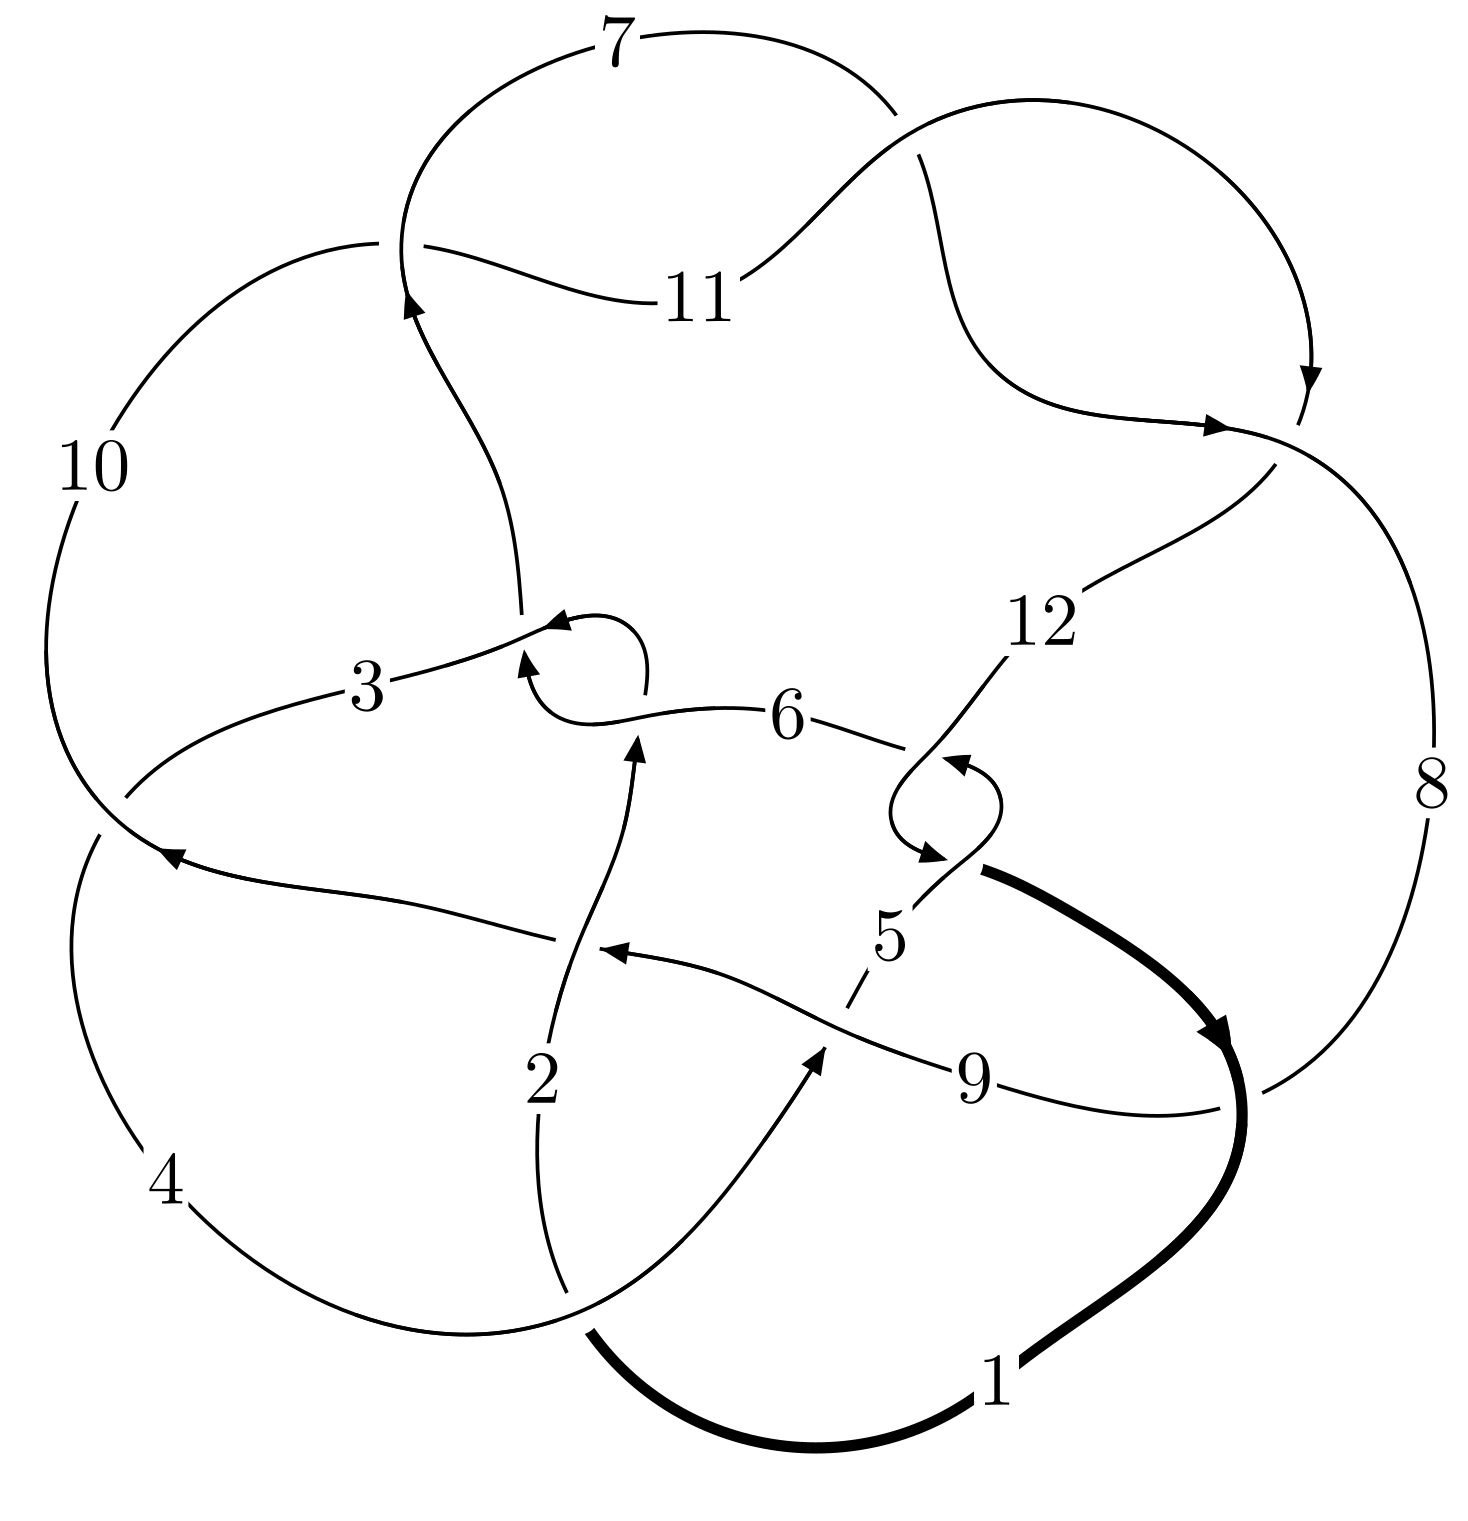
\includegraphics[width=112pt]{../../../GIT/diagram.site/Diagrams/png/1759_12a_0958.png}\\
\ \ \ A knot diagram\footnotemark}&
\allowdisplaybreaks
\textbf{Linearized knot diagam} \\
\cline{2-2}
 &
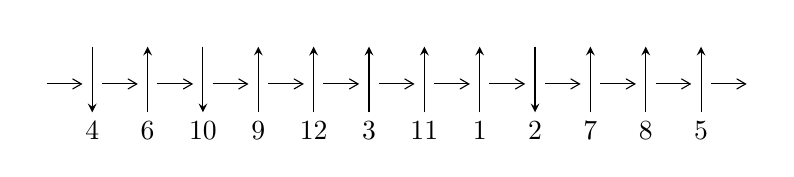
\begin{tikzpicture}[x=20pt, y=17pt]
	% nodes
	\node (C0) at (0, 0) {};
	\node (C1) at (1, 0) {};
	\node (C1U) at (1, +1) {};
	\node (C1D) at (1, -1) {4};

	\node (C2) at (2, 0) {};
	\node (C2U) at (2, +1) {};
	\node (C2D) at (2, -1) {6};

	\node (C3) at (3, 0) {};
	\node (C3U) at (3, +1) {};
	\node (C3D) at (3, -1) {10};

	\node (C4) at (4, 0) {};
	\node (C4U) at (4, +1) {};
	\node (C4D) at (4, -1) {9};

	\node (C5) at (5, 0) {};
	\node (C5U) at (5, +1) {};
	\node (C5D) at (5, -1) {12};

	\node (C6) at (6, 0) {};
	\node (C6U) at (6, +1) {};
	\node (C6D) at (6, -1) {3};

	\node (C7) at (7, 0) {};
	\node (C7U) at (7, +1) {};
	\node (C7D) at (7, -1) {11};

	\node (C8) at (8, 0) {};
	\node (C8U) at (8, +1) {};
	\node (C8D) at (8, -1) {1};

	\node (C9) at (9, 0) {};
	\node (C9U) at (9, +1) {};
	\node (C9D) at (9, -1) {2};

	\node (C10) at (10, 0) {};
	\node (C10U) at (10, +1) {};
	\node (C10D) at (10, -1) {7};

	\node (C11) at (11, 0) {};
	\node (C11U) at (11, +1) {};
	\node (C11D) at (11, -1) {8};

	\node (C12) at (12, 0) {};
	\node (C12U) at (12, +1) {};
	\node (C12D) at (12, -1) {5};
	\node (C13) at (13, 0) {};

	% arrows
	\draw[->,>={angle 60}]
	(C0) edge (C1) (C1) edge (C2) (C2) edge (C3) (C3) edge (C4) (C4) edge (C5) (C5) edge (C6) (C6) edge (C7) (C7) edge (C8) (C8) edge (C9) (C9) edge (C10) (C10) edge (C11) (C11) edge (C12) (C12) edge (C13) ;	\draw[->,>=stealth]
	(C1U) edge (C1D) (C2D) edge (C2U) (C3U) edge (C3D) (C4D) edge (C4U) (C5D) edge (C5U) (C6D) edge (C6U) (C7D) edge (C7U) (C8D) edge (C8U) (C9U) edge (C9D) (C10D) edge (C10U) (C11D) edge (C11U) (C12D) edge (C12U) ;
	\end{tikzpicture} \\
\hhline{~~} \\& 
\textbf{Solving Sequence} \\ \cline{2-2} 
 &
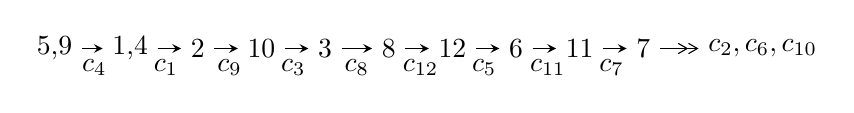
\begin{tikzpicture}[x=23pt, y=7pt]
	% node
	\node (A0) at (-1/8, 0) {5,9};
	\node (A1) at (17/16, 0) {1,4};
	\node (A2) at (17/8, 0) {2};
	\node (A3) at (25/8, 0) {10};
	\node (A4) at (33/8, 0) {3};
	\node (A5) at (41/8, 0) {8};
	\node (A6) at (49/8, 0) {12};
	\node (A7) at (57/8, 0) {6};
	\node (A8) at (65/8, 0) {11};
	\node (A9) at (73/8, 0) {7};
	\node (C1) at (1/2, -1) {$c_{4}$};
	\node (C2) at (13/8, -1) {$c_{1}$};
	\node (C3) at (21/8, -1) {$c_{9}$};
	\node (C4) at (29/8, -1) {$c_{3}$};
	\node (C5) at (37/8, -1) {$c_{8}$};
	\node (C6) at (45/8, -1) {$c_{12}$};
	\node (C7) at (53/8, -1) {$c_{5}$};
	\node (C8) at (61/8, -1) {$c_{11}$};
	\node (C9) at (69/8, -1) {$c_{7}$};
	\node (A10) at (11, 0) {$c_{2},c_{6},c_{10}$};

	% edge
	\draw[->,>=stealth]	
	(A0) edge (A1) (A1) edge (A2) (A2) edge (A3) (A3) edge (A4) (A4) edge (A5) (A5) edge (A6) (A6) edge (A7) (A7) edge (A8) (A8) edge (A9) ;
	\draw[->>,>={angle 60}]	
	(A9) edge (A10);
\end{tikzpicture} \\ 

\end{tabular} \\

\footnotetext{
The image of knot diagram is generated by the software ``\textbf{Draw programme}" developed by Andrew Bartholomew(\url{http://www.layer8.co.uk/maths/draw/index.htm\#Running-draw}), where we modified some parts for our purpose(\url{https://github.com/CATsTAILs/LinksPainter}).
}\phantom \\ \newline 
\centering \textbf{Ideals for irreducible components\footnotemark of $X_{\text{par}}$} 
 
\begin{align*}
I^u_{1}&=\langle 
3.24811\times10^{815} u^{126}-2.46551\times10^{815} u^{125}+\cdots+9.83532\times10^{817} b+9.09376\times10^{818},\\
\phantom{I^u_{1}}&\phantom{= \langle  }-1.75194\times10^{818} u^{126}-5.25120\times10^{815} u^{125}+\cdots+1.51562\times10^{821} a-1.08916\times10^{822},\\
\phantom{I^u_{1}}&\phantom{= \langle  }u^{127}- u^{126}+\cdots+17533 u+1541\rangle \\
I^u_{2}&=\langle 
-1.10098\times10^{15} u^{22}+8.50756\times10^{14} u^{21}+\cdots+6.63632\times10^{15} b+1.53110\times10^{16},\\
\phantom{I^u_{2}}&\phantom{= \langle  }4522732367957282 u^{22}-975327261831870 u^{21}+\cdots+6636320717064427 a+5366933139683854,\\
\phantom{I^u_{2}}&\phantom{= \langle  }u^{23}+8 u^{21}+\cdots-2 u+1\rangle \\
I^u_{3}&=\langle 
u^2+b+3 u+1,\;- u^2+a-4 u-4,\;u^3+3 u^2+2 u+1\rangle \\
I^u_{4}&=\langle 
b- u,\;- u^2+a+u-2,\;u^3- u^2+2 u-1\rangle \\
\\
\end{align*}
\raggedright * 4 irreducible components of $\dim_{\mathbb{C}}=0$, with total 156 representations.\\
\footnotetext{All coefficients of polynomials are rational numbers. But the coefficients are sometimes approximated in decimal forms when there is not enough margin.}
\newpage
\renewcommand{\arraystretch}{1}
\centering \section*{I. $I^u_{1}= \langle 3.25\times10^{815} u^{126}-2.47\times10^{815} u^{125}+\cdots+9.84\times10^{817} b+9.09\times10^{818},\;-1.75\times10^{818} u^{126}-5.25\times10^{815} u^{125}+\cdots+1.52\times10^{821} a-1.09\times10^{822},\;u^{127}- u^{126}+\cdots+17533 u+1541 \rangle$}
\flushleft \textbf{(i) Arc colorings}\\
\begin{tabular}{m{7pt} m{180pt} m{7pt} m{180pt} }
\flushright $a_{5}=$&$\begin{pmatrix}1\\0\end{pmatrix}$ \\
\flushright $a_{9}=$&$\begin{pmatrix}0\\u\end{pmatrix}$ \\
\flushright $a_{1}=$&$\begin{pmatrix}0.00115592 u^{126}+3.46471\times10^{-6} u^{125}+\cdots+50.3754 u+7.18625\\-0.00330250 u^{126}+0.00250680 u^{125}+\cdots-119.213 u-9.24602\end{pmatrix}$ \\
\flushright $a_{4}=$&$\begin{pmatrix}1\\u^2\end{pmatrix}$ \\
\flushright $a_{2}=$&$\begin{pmatrix}0.00477679 u^{126}-0.00358681 u^{125}+\cdots+147.480 u+14.6457\\-0.00393245 u^{126}+0.00319957 u^{125}+\cdots-125.329 u-9.29317\end{pmatrix}$ \\
\flushright $a_{10}=$&$\begin{pmatrix}-0.00686858 u^{126}+0.0127713 u^{125}+\cdots+464.976 u+54.0429\\0.000983727 u^{126}-0.00205194 u^{125}+\cdots-136.835 u-14.3804\end{pmatrix}$ \\
\flushright $a_{3}=$&$\begin{pmatrix}0.0156371 u^{126}-0.0127997 u^{125}+\cdots+573.026 u+44.8327\\-0.00738456 u^{126}+0.00721566 u^{125}+\cdots-281.515 u-20.3776\end{pmatrix}$ \\
\flushright $a_{8}=$&$\begin{pmatrix}-0.00750345 u^{126}+0.0130698 u^{125}+\cdots+405.454 u+47.2377\\0.00108359 u^{126}-0.00196659 u^{125}+\cdots-99.6256 u-10.0985\end{pmatrix}$ \\
\flushright $a_{12}=$&$\begin{pmatrix}0.00445842 u^{126}-0.00250333 u^{125}+\cdots+169.589 u+16.4323\\-0.00330250 u^{126}+0.00250680 u^{125}+\cdots-119.213 u-9.24602\end{pmatrix}$ \\
\flushright $a_{6}=$&$\begin{pmatrix}0.0100270 u^{126}-0.00862773 u^{125}+\cdots+375.684 u+28.8926\\-0.00347385 u^{126}+0.00315813 u^{125}+\cdots-186.725 u-13.6212\end{pmatrix}$ \\
\flushright $a_{11}=$&$\begin{pmatrix}-0.00496870 u^{126}+0.000885001 u^{125}+\cdots-378.517 u-36.7701\\0.000661809 u^{126}+0.000354500 u^{125}+\cdots+63.5886 u+6.17548\end{pmatrix}$ \\
\flushright $a_{7}=$&$\begin{pmatrix}-0.00506831 u^{126}+0.00355203 u^{125}+\cdots-219.198 u-13.1992\\0.00335759 u^{126}-0.00443429 u^{125}+\cdots+58.2261 u+3.86702\end{pmatrix}$\\&\end{tabular}
\flushleft \textbf{(ii) Obstruction class $= -1$}\\~\\
\flushleft \textbf{(iii) Cusp Shapes $= -0.0123516 u^{126}-0.00278997 u^{125}+\cdots-1942.80 u-202.679$}\\~\\
\newpage\renewcommand{\arraystretch}{1}
\flushleft \textbf{(iv) u-Polynomials at the component}\newline \\
\begin{tabular}{m{50pt}|m{274pt}}
Crossings & \hspace{64pt}u-Polynomials at each crossing \\
\hline $$\begin{aligned}c_{1}\end{aligned}$$&$\begin{aligned}
&u^{127}-5 u^{126}+\cdots-1344 u+64
\end{aligned}$\\
\hline $$\begin{aligned}c_{2},c_{6}\end{aligned}$$&$\begin{aligned}
&u^{127}+2 u^{126}+\cdots+10323 u+2467
\end{aligned}$\\
\hline $$\begin{aligned}c_{3}\end{aligned}$$&$\begin{aligned}
&u^{127}-3 u^{126}+\cdots+1233985982 u-292939631
\end{aligned}$\\
\hline $$\begin{aligned}c_{4}\end{aligned}$$&$\begin{aligned}
&u^{127}+u^{126}+\cdots+17533 u-1541
\end{aligned}$\\
\hline $$\begin{aligned}c_{5},c_{12}\end{aligned}$$&$\begin{aligned}
&u^{127}+3 u^{126}+\cdots-39833 u+3461
\end{aligned}$\\
\hline $$\begin{aligned}c_{7},c_{10},c_{11}\end{aligned}$$&$\begin{aligned}
&u^{127}-5 u^{126}+\cdots-361 u+29
\end{aligned}$\\
\hline $$\begin{aligned}c_{8}\end{aligned}$$&$\begin{aligned}
&u^{127}+u^{126}+\cdots-26 u-1
\end{aligned}$\\
\hline $$\begin{aligned}c_{9}\end{aligned}$$&$\begin{aligned}
&u^{127}- u^{126}+\cdots+3405 u+207
\end{aligned}$\\
\hline
\end{tabular}\\~\\
\newpage\renewcommand{\arraystretch}{1}
\flushleft \textbf{(v) Riley Polynomials at the component}\newline \\
\begin{tabular}{m{50pt}|m{274pt}}
Crossings & \hspace{64pt}Riley Polynomials at each crossing \\
\hline $$\begin{aligned}c_{1}\end{aligned}$$&$\begin{aligned}
&y^{127}+5 y^{126}+\cdots+215040 y-4096
\end{aligned}$\\
\hline $$\begin{aligned}c_{2},c_{6}\end{aligned}$$&$\begin{aligned}
&y^{127}-82 y^{126}+\cdots+357241133 y-6086089
\end{aligned}$\\
\hline $$\begin{aligned}c_{3}\end{aligned}$$&$\begin{aligned}
&y^{127}+37 y^{126}+\cdots-3665675937186530842 y-85813627410416161
\end{aligned}$\\
\hline $$\begin{aligned}c_{4}\end{aligned}$$&$\begin{aligned}
&y^{127}+35 y^{126}+\cdots+35832577 y-2374681
\end{aligned}$\\
\hline $$\begin{aligned}c_{5},c_{12}\end{aligned}$$&$\begin{aligned}
&y^{127}+61 y^{126}+\cdots+1408883241 y-11978521
\end{aligned}$\\
\hline $$\begin{aligned}c_{7},c_{10},c_{11}\end{aligned}$$&$\begin{aligned}
&y^{127}-141 y^{126}+\cdots+115183 y-841
\end{aligned}$\\
\hline $$\begin{aligned}c_{8}\end{aligned}$$&$\begin{aligned}
&y^{127}+y^{126}+\cdots+116 y-1
\end{aligned}$\\
\hline $$\begin{aligned}c_{9}\end{aligned}$$&$\begin{aligned}
&y^{127}-13 y^{126}+\cdots+5912703 y-42849
\end{aligned}$\\
\hline
\end{tabular}\\~\\
\newpage\flushleft \textbf{(vi) Complex Volumes and Cusp Shapes}
$$\begin{array}{c|c|c}  
\text{Solutions to }I^u_{1}& \I (\text{vol} + \sqrt{-1}CS) & \text{Cusp shape}\\
 \hline 
\begin{aligned}
u &= -0.454897 + 0.911052 I \\
a &= \phantom{-}1.236380 + 0.261261 I \\
b &= -0.089606 - 0.913498 I\end{aligned}
 & \phantom{-}0.559126 + 0.625580 I & \phantom{-0.000000 } 0 \\ \hline\begin{aligned}
u &= -0.454897 - 0.911052 I \\
a &= \phantom{-}1.236380 - 0.261261 I \\
b &= -0.089606 + 0.913498 I\end{aligned}
 & \phantom{-}0.559126 - 0.625580 I & \phantom{-0.000000 } 0 \\ \hline\begin{aligned}
u &= \phantom{-}0.364851 + 0.905528 I \\
a &= \phantom{-}0.903144 - 0.657744 I \\
b &= \phantom{-}0.203950 + 1.280870 I\end{aligned}
 & -3.19098 + 2.67904 I & \phantom{-0.000000 } 0 \\ \hline\begin{aligned}
u &= \phantom{-}0.364851 - 0.905528 I \\
a &= \phantom{-}0.903144 + 0.657744 I \\
b &= \phantom{-}0.203950 - 1.280870 I\end{aligned}
 & -3.19098 - 2.67904 I & \phantom{-0.000000 } 0 \\ \hline\begin{aligned}
u &= -0.964069\phantom{ +0.000000I} \\
a &= \phantom{-}0.535737\phantom{ +0.000000I} \\
b &= \phantom{-}0.630821\phantom{ +0.000000I}\end{aligned}
 & \phantom{-}1.16343\phantom{ +0.000000I} & \phantom{-0.000000 } 0 \\ \hline\begin{aligned}
u &= \phantom{-}0.353449 + 0.888121 I \\
a &= \phantom{-}0.940412 - 0.922540 I \\
b &= \phantom{-}0.178902 + 1.286600 I\end{aligned}
 & -3.18398 + 2.66953 I & \phantom{-0.000000 } 0 \\ \hline\begin{aligned}
u &= \phantom{-}0.353449 - 0.888121 I \\
a &= \phantom{-}0.940412 + 0.922540 I \\
b &= \phantom{-}0.178902 - 1.286600 I\end{aligned}
 & -3.18398 - 2.66953 I & \phantom{-0.000000 } 0 \\ \hline\begin{aligned}
u &= \phantom{-}1.055390 + 0.142832 I \\
a &= \phantom{-}0.348792 - 0.167075 I \\
b &= \phantom{-}0.240369 - 0.821665 I\end{aligned}
 & -0.35427 - 2.07951 I & \phantom{-0.000000 } 0 \\ \hline\begin{aligned}
u &= \phantom{-}1.055390 - 0.142832 I \\
a &= \phantom{-}0.348792 + 0.167075 I \\
b &= \phantom{-}0.240369 + 0.821665 I\end{aligned}
 & -0.35427 + 2.07951 I & \phantom{-0.000000 } 0 \\ \hline\begin{aligned}
u &= -0.304445 + 0.880878 I \\
a &= \phantom{-}1.202040 + 0.207316 I \\
b &= \phantom{-}0.52487 - 1.33794 I\end{aligned}
 & -2.09198 - 6.77319 I & \phantom{-0.000000 } 0\\
 \hline 
 \end{array}$$\newpage$$\begin{array}{c|c|c}  
\text{Solutions to }I^u_{1}& \I (\text{vol} + \sqrt{-1}CS) & \text{Cusp shape}\\
 \hline 
\begin{aligned}
u &= -0.304445 - 0.880878 I \\
a &= \phantom{-}1.202040 - 0.207316 I \\
b &= \phantom{-}0.52487 + 1.33794 I\end{aligned}
 & -2.09198 + 6.77319 I & \phantom{-0.000000 } 0 \\ \hline\begin{aligned}
u &= \phantom{-}0.632797 + 0.650968 I \\
a &= \phantom{-}0.724983 + 0.404447 I \\
b &= \phantom{-}1.15491 + 0.96814 I\end{aligned}
 & \phantom{-}7.33318 - 2.03058 I & \phantom{-0.000000 } 0 \\ \hline\begin{aligned}
u &= \phantom{-}0.632797 - 0.650968 I \\
a &= \phantom{-}0.724983 - 0.404447 I \\
b &= \phantom{-}1.15491 - 0.96814 I\end{aligned}
 & \phantom{-}7.33318 + 2.03058 I & \phantom{-0.000000 } 0 \\ \hline\begin{aligned}
u &= \phantom{-}0.612874 + 0.663367 I \\
a &= -0.587697 - 0.297157 I \\
b &= -0.488503 + 0.291381 I\end{aligned}
 & -1.15905 + 1.71609 I & \phantom{-0.000000 } 0 \\ \hline\begin{aligned}
u &= \phantom{-}0.612874 - 0.663367 I \\
a &= -0.587697 + 0.297157 I \\
b &= -0.488503 - 0.291381 I\end{aligned}
 & -1.15905 - 1.71609 I & \phantom{-0.000000 } 0 \\ \hline\begin{aligned}
u &= -0.537008 + 0.717718 I \\
a &= \phantom{-}1.36776 + 0.49896 I \\
b &= \phantom{-}0.934426 + 0.402625 I\end{aligned}
 & \phantom{-}11.89500 + 0.48258 I & \phantom{-0.000000 } 0 \\ \hline\begin{aligned}
u &= -0.537008 - 0.717718 I \\
a &= \phantom{-}1.36776 - 0.49896 I \\
b &= \phantom{-}0.934426 - 0.402625 I\end{aligned}
 & \phantom{-}11.89500 - 0.48258 I & \phantom{-0.000000 } 0 \\ \hline\begin{aligned}
u &= -0.669529 + 0.880014 I \\
a &= -0.849664 - 0.146800 I \\
b &= -0.758023 - 0.071047 I\end{aligned}
 & \phantom{-}0.20746 - 4.43767 I & \phantom{-0.000000 } 0 \\ \hline\begin{aligned}
u &= -0.669529 - 0.880014 I \\
a &= -0.849664 + 0.146800 I \\
b &= -0.758023 + 0.071047 I\end{aligned}
 & \phantom{-}0.20746 + 4.43767 I & \phantom{-0.000000 } 0 \\ \hline\begin{aligned}
u &= \phantom{-}0.745732 + 0.817700 I \\
a &= \phantom{-}1.33611 + 0.83979 I \\
b &= -0.181688 + 0.806349 I\end{aligned}
 & \phantom{-}7.25608 + 6.95311 I & \phantom{-0.000000 } 0\\
 \hline 
 \end{array}$$\newpage$$\begin{array}{c|c|c}  
\text{Solutions to }I^u_{1}& \I (\text{vol} + \sqrt{-1}CS) & \text{Cusp shape}\\
 \hline 
\begin{aligned}
u &= \phantom{-}0.745732 - 0.817700 I \\
a &= \phantom{-}1.33611 - 0.83979 I \\
b &= -0.181688 - 0.806349 I\end{aligned}
 & \phantom{-}7.25608 - 6.95311 I & \phantom{-0.000000 } 0 \\ \hline\begin{aligned}
u &= \phantom{-}0.246295 + 0.856716 I \\
a &= \phantom{-}1.44391 - 0.09789 I \\
b &= \phantom{-}0.78232 + 1.30470 I\end{aligned}
 & \phantom{-}5.44496 + 9.85386 I & \phantom{-0.000000 } 0 \\ \hline\begin{aligned}
u &= \phantom{-}0.246295 - 0.856716 I \\
a &= \phantom{-}1.44391 + 0.09789 I \\
b &= \phantom{-}0.78232 - 1.30470 I\end{aligned}
 & \phantom{-}5.44496 - 9.85386 I & \phantom{-0.000000 } 0 \\ \hline\begin{aligned}
u &= -0.034823 + 0.889992 I \\
a &= -0.921638 - 0.430012 I \\
b &= -0.136518 + 1.160520 I\end{aligned}
 & -3.73206 + 1.61429 I & \phantom{-0.000000 } 0 \\ \hline\begin{aligned}
u &= -0.034823 - 0.889992 I \\
a &= -0.921638 + 0.430012 I \\
b &= -0.136518 - 1.160520 I\end{aligned}
 & -3.73206 - 1.61429 I & \phantom{-0.000000 } 0 \\ \hline\begin{aligned}
u &= -0.724488 + 0.510499 I \\
a &= -0.042859 - 0.169584 I \\
b &= -0.84523 - 1.18019 I\end{aligned}
 & \phantom{-}3.13816 + 0.66185 I & \phantom{-0.000000 } 0 \\ \hline\begin{aligned}
u &= -0.724488 - 0.510499 I \\
a &= -0.042859 + 0.169584 I \\
b &= -0.84523 + 1.18019 I\end{aligned}
 & \phantom{-}3.13816 - 0.66185 I & \phantom{-0.000000 } 0 \\ \hline\begin{aligned}
u &= -0.309997 + 0.826021 I \\
a &= \phantom{-}1.38789 + 1.88410 I \\
b &= \phantom{-}0.19953 - 1.47411 I\end{aligned}
 & \phantom{-}1.64868 - 4.08208 I & \phantom{-0.000000 } 0 \\ \hline\begin{aligned}
u &= -0.309997 - 0.826021 I \\
a &= \phantom{-}1.38789 - 1.88410 I \\
b &= \phantom{-}0.19953 + 1.47411 I\end{aligned}
 & \phantom{-}1.64868 + 4.08208 I & \phantom{-0.000000 } 0 \\ \hline\begin{aligned}
u &= -0.242034 + 0.841163 I \\
a &= -0.59511 + 1.58495 I \\
b &= \phantom{-}0.313244 - 0.932375 I\end{aligned}
 & \phantom{-}3.30458 - 2.00993 I & \phantom{-0.000000 } 0\\
 \hline 
 \end{array}$$\newpage$$\begin{array}{c|c|c}  
\text{Solutions to }I^u_{1}& \I (\text{vol} + \sqrt{-1}CS) & \text{Cusp shape}\\
 \hline 
\begin{aligned}
u &= -0.242034 - 0.841163 I \\
a &= -0.59511 - 1.58495 I \\
b &= \phantom{-}0.313244 + 0.932375 I\end{aligned}
 & \phantom{-}3.30458 + 2.00993 I & \phantom{-0.000000 } 0 \\ \hline\begin{aligned}
u &= \phantom{-}0.926532 + 0.637758 I \\
a &= -1.58255 - 0.25843 I \\
b &= -0.483025 - 1.252390 I\end{aligned}
 & \phantom{-}9.65313 + 9.05864 I & \phantom{-0.000000 } 0 \\ \hline\begin{aligned}
u &= \phantom{-}0.926532 - 0.637758 I \\
a &= -1.58255 + 0.25843 I \\
b &= -0.483025 + 1.252390 I\end{aligned}
 & \phantom{-}9.65313 - 9.05864 I & \phantom{-0.000000 } 0 \\ \hline\begin{aligned}
u &= -0.765524 + 0.403805 I \\
a &= -1.56302 - 0.22468 I \\
b &= -0.872536 - 0.167249 I\end{aligned}
 & \phantom{-}13.05490 - 4.10370 I & \phantom{-0.000000 } 0 \\ \hline\begin{aligned}
u &= -0.765524 - 0.403805 I \\
a &= -1.56302 + 0.22468 I \\
b &= -0.872536 + 0.167249 I\end{aligned}
 & \phantom{-}13.05490 + 4.10370 I & \phantom{-0.000000 } 0 \\ \hline\begin{aligned}
u &= \phantom{-}0.842786 + 0.760771 I \\
a &= \phantom{-}0.872088 - 0.638158 I \\
b &= \phantom{-}0.914725 + 0.316028 I\end{aligned}
 & \phantom{-}7.85544 + 0.11358 I & \phantom{-0.000000 } 0 \\ \hline\begin{aligned}
u &= \phantom{-}0.842786 - 0.760771 I \\
a &= \phantom{-}0.872088 + 0.638158 I \\
b &= \phantom{-}0.914725 - 0.316028 I\end{aligned}
 & \phantom{-}7.85544 - 0.11358 I & \phantom{-0.000000 } 0 \\ \hline\begin{aligned}
u &= \phantom{-}0.841248 + 0.047036 I \\
a &= -1.084480 - 0.673211 I \\
b &= -0.588181 + 0.238816 I\end{aligned}
 & \phantom{-}4.87440 + 0.69256 I & \phantom{-0.000000 } 0 \\ \hline\begin{aligned}
u &= \phantom{-}0.841248 - 0.047036 I \\
a &= -1.084480 + 0.673211 I \\
b &= -0.588181 - 0.238816 I\end{aligned}
 & \phantom{-}4.87440 - 0.69256 I & \phantom{-0.000000 } 0 \\ \hline\begin{aligned}
u &= -0.944043 + 0.688858 I \\
a &= \phantom{-}0.529722 - 0.529388 I \\
b &= \phantom{-}0.1209810 - 0.0073066 I\end{aligned}
 & \phantom{-}2.75448 - 4.67938 I & \phantom{-0.000000 } 0\\
 \hline 
 \end{array}$$\newpage$$\begin{array}{c|c|c}  
\text{Solutions to }I^u_{1}& \I (\text{vol} + \sqrt{-1}CS) & \text{Cusp shape}\\
 \hline 
\begin{aligned}
u &= -0.944043 - 0.688858 I \\
a &= \phantom{-}0.529722 + 0.529388 I \\
b &= \phantom{-}0.1209810 + 0.0073066 I\end{aligned}
 & \phantom{-}2.75448 + 4.67938 I & \phantom{-0.000000 } 0 \\ \hline\begin{aligned}
u &= -0.654357 + 0.484227 I \\
a &= \phantom{-}0.821743 + 0.225535 I \\
b &= \phantom{-}0.391190 - 0.102487 I\end{aligned}
 & \phantom{-}1.076060 - 0.369429 I & \phantom{-0.000000 } 0 \\ \hline\begin{aligned}
u &= -0.654357 - 0.484227 I \\
a &= \phantom{-}0.821743 - 0.225535 I \\
b &= \phantom{-}0.391190 + 0.102487 I\end{aligned}
 & \phantom{-}1.076060 + 0.369429 I & \phantom{-0.000000 } 0 \\ \hline\begin{aligned}
u &= \phantom{-}0.762044 + 0.916108 I \\
a &= -0.004572 + 0.615664 I \\
b &= -0.360453 + 1.027130 I\end{aligned}
 & \phantom{-}9.20578 + 0.95990 I & \phantom{-0.000000 } 0 \\ \hline\begin{aligned}
u &= \phantom{-}0.762044 - 0.916108 I \\
a &= -0.004572 - 0.615664 I \\
b &= -0.360453 - 1.027130 I\end{aligned}
 & \phantom{-}9.20578 - 0.95990 I & \phantom{-0.000000 } 0 \\ \hline\begin{aligned}
u &= -1.100180 + 0.460924 I \\
a &= \phantom{-}0.349419 + 0.461107 I \\
b &= \phantom{-}0.546703 + 1.099350 I\end{aligned}
 & \phantom{-}5.42405 + 5.10393 I & \phantom{-0.000000 } 0 \\ \hline\begin{aligned}
u &= -1.100180 - 0.460924 I \\
a &= \phantom{-}0.349419 - 0.461107 I \\
b &= \phantom{-}0.546703 - 1.099350 I\end{aligned}
 & \phantom{-}5.42405 - 5.10393 I & \phantom{-0.000000 } 0 \\ \hline\begin{aligned}
u &= -0.828021 + 0.862047 I \\
a &= \phantom{-}1.278050 - 0.252875 I \\
b &= \phantom{-}0.462587 - 0.860582 I\end{aligned}
 & \phantom{-}3.00752 - 5.37604 I & \phantom{-0.000000 } 0 \\ \hline\begin{aligned}
u &= -0.828021 - 0.862047 I \\
a &= \phantom{-}1.278050 + 0.252875 I \\
b &= \phantom{-}0.462587 + 0.860582 I\end{aligned}
 & \phantom{-}3.00752 + 5.37604 I & \phantom{-0.000000 } 0 \\ \hline\begin{aligned}
u &= \phantom{-}0.803669 + 0.893064 I \\
a &= \phantom{-}1.59245 + 0.06065 I \\
b &= \phantom{-}0.560675 + 1.197540 I\end{aligned}
 & \phantom{-}9.28090 + 4.98514 I & \phantom{-0.000000 } 0\\
 \hline 
 \end{array}$$\newpage$$\begin{array}{c|c|c}  
\text{Solutions to }I^u_{1}& \I (\text{vol} + \sqrt{-1}CS) & \text{Cusp shape}\\
 \hline 
\begin{aligned}
u &= \phantom{-}0.803669 - 0.893064 I \\
a &= \phantom{-}1.59245 - 0.06065 I \\
b &= \phantom{-}0.560675 - 1.197540 I\end{aligned}
 & \phantom{-}9.28090 - 4.98514 I & \phantom{-0.000000 } 0 \\ \hline\begin{aligned}
u &= \phantom{-}0.755494 + 0.938460 I \\
a &= -0.881408 + 0.391019 I \\
b &= -1.145520 + 0.049576 I\end{aligned}
 & \phantom{-}7.29999 + 5.77567 I & \phantom{-0.000000 } 0 \\ \hline\begin{aligned}
u &= \phantom{-}0.755494 - 0.938460 I \\
a &= -0.881408 - 0.391019 I \\
b &= -1.145520 - 0.049576 I\end{aligned}
 & \phantom{-}7.29999 - 5.77567 I & \phantom{-0.000000 } 0 \\ \hline\begin{aligned}
u &= \phantom{-}0.182060 + 0.773412 I \\
a &= -1.59807 - 0.01138 I \\
b &= -0.387588 - 1.135120 I\end{aligned}
 & -4.73202 + 1.17378 I & \phantom{-0.000000 } 0 \\ \hline\begin{aligned}
u &= \phantom{-}0.182060 - 0.773412 I \\
a &= -1.59807 + 0.01138 I \\
b &= -0.387588 + 1.135120 I\end{aligned}
 & -4.73202 - 1.17378 I & \phantom{-0.000000 } 0 \\ \hline\begin{aligned}
u &= -0.314902 + 0.722477 I \\
a &= -2.90582 + 0.44698 I \\
b &= \phantom{-}0.154572 + 0.948395 I\end{aligned}
 & \phantom{-}1.41058 + 0.66806 I & \phantom{-0.000000 } 0 \\ \hline\begin{aligned}
u &= -0.314902 - 0.722477 I \\
a &= -2.90582 - 0.44698 I \\
b &= \phantom{-}0.154572 - 0.948395 I\end{aligned}
 & \phantom{-}1.41058 - 0.66806 I & \phantom{-0.000000 } 0 \\ \hline\begin{aligned}
u &= -0.231689 + 0.741214 I \\
a &= -1.73699 + 0.50596 I \\
b &= -0.721990 + 1.036050 I\end{aligned}
 & \phantom{-}1.32567 - 2.90614 I & \phantom{-0.000000 } 0 \\ \hline\begin{aligned}
u &= -0.231689 - 0.741214 I \\
a &= -1.73699 - 0.50596 I \\
b &= -0.721990 - 1.036050 I\end{aligned}
 & \phantom{-}1.32567 + 2.90614 I & \phantom{-0.000000 } 0 \\ \hline\begin{aligned}
u &= -0.896987 + 0.860662 I \\
a &= \phantom{-}0.843915 + 0.201618 I \\
b &= \phantom{-}1.401600 + 0.112990 I\end{aligned}
 & \phantom{-}11.6518 - 11.7658 I & \phantom{-0.000000 } 0\\
 \hline 
 \end{array}$$\newpage$$\begin{array}{c|c|c}  
\text{Solutions to }I^u_{1}& \I (\text{vol} + \sqrt{-1}CS) & \text{Cusp shape}\\
 \hline 
\begin{aligned}
u &= -0.896987 - 0.860662 I \\
a &= \phantom{-}0.843915 - 0.201618 I \\
b &= \phantom{-}1.401600 - 0.112990 I\end{aligned}
 & \phantom{-}11.6518 + 11.7658 I & \phantom{-0.000000 } 0 \\ \hline\begin{aligned}
u &= \phantom{-}0.916351 + 0.859472 I \\
a &= \phantom{-}0.829089 - 0.033001 I \\
b &= \phantom{-}1.049720 + 0.101056 I\end{aligned}
 & \phantom{-}4.38768 + 8.69266 I & \phantom{-0.000000 } 0 \\ \hline\begin{aligned}
u &= \phantom{-}0.916351 - 0.859472 I \\
a &= \phantom{-}0.829089 + 0.033001 I \\
b &= \phantom{-}1.049720 - 0.101056 I\end{aligned}
 & \phantom{-}4.38768 - 8.69266 I & \phantom{-0.000000 } 0 \\ \hline\begin{aligned}
u &= \phantom{-}0.257071 + 0.670014 I \\
a &= -2.73889 + 0.10092 I \\
b &= -0.111502 - 1.044230 I\end{aligned}
 & -4.25279 + 0.60258 I & \phantom{-0.000000 -}0. + 7.99103 I \\ \hline\begin{aligned}
u &= \phantom{-}0.257071 - 0.670014 I \\
a &= -2.73889 - 0.10092 I \\
b &= -0.111502 + 1.044230 I\end{aligned}
 & -4.25279 - 0.60258 I & \phantom{-0.000000 } 0. - 7.99103 I \\ \hline\begin{aligned}
u &= -0.079891 + 1.294470 I \\
a &= \phantom{-}0.112299 - 1.369410 I \\
b &= -0.131679 + 0.805279 I\end{aligned}
 & \phantom{-}10.47890 - 3.07948 I & \phantom{-0.000000 } 0 \\ \hline\begin{aligned}
u &= -0.079891 - 1.294470 I \\
a &= \phantom{-}0.112299 + 1.369410 I \\
b &= -0.131679 - 0.805279 I\end{aligned}
 & \phantom{-}10.47890 + 3.07948 I & \phantom{-0.000000 } 0 \\ \hline\begin{aligned}
u &= \phantom{-}0.490618 + 0.493448 I \\
a &= \phantom{-}1.136370 - 0.072984 I \\
b &= \phantom{-}0.972754 - 0.617116 I\end{aligned}
 & \phantom{-}3.68376 + 0.15468 I & \phantom{-}13.04643 - 5.18596 I \\ \hline\begin{aligned}
u &= \phantom{-}0.490618 - 0.493448 I \\
a &= \phantom{-}1.136370 + 0.072984 I \\
b &= \phantom{-}0.972754 + 0.617116 I\end{aligned}
 & \phantom{-}3.68376 - 0.15468 I & \phantom{-}13.04643 + 5.18596 I \\ \hline\begin{aligned}
u &= -0.442393 + 0.530026 I \\
a &= \phantom{-}0.662775 - 0.185174 I \\
b &= \phantom{-}1.096030 - 0.379727 I\end{aligned}
 & \phantom{-}1.67691 + 0.65702 I & \phantom{-}1.51745 + 4.11768 I\\
 \hline 
 \end{array}$$\newpage$$\begin{array}{c|c|c}  
\text{Solutions to }I^u_{1}& \I (\text{vol} + \sqrt{-1}CS) & \text{Cusp shape}\\
 \hline 
\begin{aligned}
u &= -0.442393 - 0.530026 I \\
a &= \phantom{-}0.662775 + 0.185174 I \\
b &= \phantom{-}1.096030 + 0.379727 I\end{aligned}
 & \phantom{-}1.67691 - 0.65702 I & \phantom{-}1.51745 - 4.11768 I \\ \hline\begin{aligned}
u &= -0.777622 + 1.149890 I \\
a &= \phantom{-}0.038656 - 0.268231 I \\
b &= -0.195483 - 0.459087 I\end{aligned}
 & \phantom{-}2.45396 - 0.71763 I & \phantom{-0.000000 } 0 \\ \hline\begin{aligned}
u &= -0.777622 - 1.149890 I \\
a &= \phantom{-}0.038656 + 0.268231 I \\
b &= -0.195483 + 0.459087 I\end{aligned}
 & \phantom{-}2.45396 + 0.71763 I & \phantom{-0.000000 } 0 \\ \hline\begin{aligned}
u &= -0.005560 + 0.609730 I \\
a &= \phantom{-}3.28949 - 1.62600 I \\
b &= -0.224196 + 1.006980 I\end{aligned}
 & \phantom{-}6.49113 - 8.79984 I & \phantom{-}4.45971 + 5.72952 I \\ \hline\begin{aligned}
u &= -0.005560 - 0.609730 I \\
a &= \phantom{-}3.28949 + 1.62600 I \\
b &= -0.224196 - 1.006980 I\end{aligned}
 & \phantom{-}6.49113 + 8.79984 I & \phantom{-}4.45971 - 5.72952 I \\ \hline\begin{aligned}
u &= -1.254060 + 0.624367 I \\
a &= -0.818721 + 0.391812 I \\
b &= -0.357603 + 1.079120 I\end{aligned}
 & \phantom{-}2.47405 - 4.31871 I & \phantom{-0.000000 } 0 \\ \hline\begin{aligned}
u &= -1.254060 - 0.624367 I \\
a &= -0.818721 - 0.391812 I \\
b &= -0.357603 - 1.079120 I\end{aligned}
 & \phantom{-}2.47405 + 4.31871 I & \phantom{-0.000000 } 0 \\ \hline\begin{aligned}
u &= -0.875330 + 1.096280 I \\
a &= \phantom{-}0.994591 + 0.148767 I \\
b &= \phantom{-}0.69277 - 1.35605 I\end{aligned}
 & \phantom{-}1.06463 - 7.82295 I & \phantom{-0.000000 } 0 \\ \hline\begin{aligned}
u &= -0.875330 - 1.096280 I \\
a &= \phantom{-}0.994591 - 0.148767 I \\
b &= \phantom{-}0.69277 + 1.35605 I\end{aligned}
 & \phantom{-}1.06463 + 7.82295 I & \phantom{-0.000000 } 0 \\ \hline\begin{aligned}
u &= \phantom{-}0.731462 + 1.206850 I \\
a &= \phantom{-}0.894000 - 0.269771 I \\
b &= \phantom{-}0.393242 + 1.272140 I\end{aligned}
 & -3.24017 + 3.59589 I & \phantom{-0.000000 } 0\\
 \hline 
 \end{array}$$\newpage$$\begin{array}{c|c|c}  
\text{Solutions to }I^u_{1}& \I (\text{vol} + \sqrt{-1}CS) & \text{Cusp shape}\\
 \hline 
\begin{aligned}
u &= \phantom{-}0.731462 - 1.206850 I \\
a &= \phantom{-}0.894000 + 0.269771 I \\
b &= \phantom{-}0.393242 - 1.272140 I\end{aligned}
 & -3.24017 - 3.59589 I & \phantom{-0.000000 } 0 \\ \hline\begin{aligned}
u &= -0.88236 + 1.11457 I \\
a &= -0.492130 - 0.691183 I \\
b &= -0.834998 + 0.681281 I\end{aligned}
 & \phantom{-}11.01530 + 5.14924 I & \phantom{-0.000000 } 0 \\ \hline\begin{aligned}
u &= -0.88236 - 1.11457 I \\
a &= -0.492130 + 0.691183 I \\
b &= -0.834998 - 0.681281 I\end{aligned}
 & \phantom{-}11.01530 - 5.14924 I & \phantom{-0.000000 } 0 \\ \hline\begin{aligned}
u &= \phantom{-}0.571916\phantom{ +0.000000I} \\
a &= \phantom{-}0.777170\phantom{ +0.000000I} \\
b &= \phantom{-}2.15862\phantom{ +0.000000I}\end{aligned}
 & \phantom{-}4.54867\phantom{ +0.000000I} & \phantom{-}34.0560\phantom{ +0.000000I} \\ \hline\begin{aligned}
u &= -0.80299 + 1.19060 I \\
a &= -1.253900 - 0.293786 I \\
b &= -0.59518 + 1.34906 I\end{aligned}
 & \phantom{-}3.28531 - 11.90180 I & \phantom{-0.000000 } 0 \\ \hline\begin{aligned}
u &= -0.80299 - 1.19060 I \\
a &= -1.253900 + 0.293786 I \\
b &= -0.59518 - 1.34906 I\end{aligned}
 & \phantom{-}3.28531 + 11.90180 I & \phantom{-0.000000 } 0 \\ \hline\begin{aligned}
u &= \phantom{-}0.028522 + 0.532814 I \\
a &= \phantom{-}2.59823 + 2.19202 I \\
b &= -0.092222 - 1.166290 I\end{aligned}
 & -0.49895 + 5.51266 I & \phantom{-}3.87288 - 8.41207 I \\ \hline\begin{aligned}
u &= \phantom{-}0.028522 - 0.532814 I \\
a &= \phantom{-}2.59823 - 2.19202 I \\
b &= -0.092222 + 1.166290 I\end{aligned}
 & -0.49895 - 5.51266 I & \phantom{-}3.87288 + 8.41207 I \\ \hline\begin{aligned}
u &= -0.41618 + 1.42484 I \\
a &= \phantom{-}0.639655 + 0.556368 I \\
b &= \phantom{-}0.114977 - 1.126460 I\end{aligned}
 & -0.100427 + 1.151540 I & \phantom{-0.000000 } 0 \\ \hline\begin{aligned}
u &= -0.41618 - 1.42484 I \\
a &= \phantom{-}0.639655 - 0.556368 I \\
b &= \phantom{-}0.114977 + 1.126460 I\end{aligned}
 & -0.100427 - 1.151540 I & \phantom{-0.000000 } 0\\
 \hline 
 \end{array}$$\newpage$$\begin{array}{c|c|c}  
\text{Solutions to }I^u_{1}& \I (\text{vol} + \sqrt{-1}CS) & \text{Cusp shape}\\
 \hline 
\begin{aligned}
u &= -0.191192 + 0.478084 I \\
a &= -3.57333 - 1.96870 I \\
b &= -0.227655 + 1.258130 I\end{aligned}
 & -1.59523 - 2.47874 I & -1.76895 - 3.57372 I \\ \hline\begin{aligned}
u &= -0.191192 - 0.478084 I \\
a &= -3.57333 + 1.96870 I \\
b &= -0.227655 - 1.258130 I\end{aligned}
 & -1.59523 + 2.47874 I & -1.76895 + 3.57372 I \\ \hline\begin{aligned}
u &= \phantom{-}0.81001 + 1.25615 I \\
a &= -1.066650 + 0.241770 I \\
b &= -0.454020 - 1.234480 I\end{aligned}
 & -3.31619 + 8.92992 I & \phantom{-0.000000 } 0 \\ \hline\begin{aligned}
u &= \phantom{-}0.81001 - 1.25615 I \\
a &= -1.066650 - 0.241770 I \\
b &= -0.454020 + 1.234480 I\end{aligned}
 & -3.31619 - 8.92992 I & \phantom{-0.000000 } 0 \\ \hline\begin{aligned}
u &= \phantom{-}0.503512\phantom{ +0.000000I} \\
a &= -0.379845\phantom{ +0.000000I} \\
b &= -2.53263\phantom{ +0.000000I}\end{aligned}
 & -0.427603\phantom{ +0.000000I} & \phantom{-}295.740\phantom{ +0.000000I} \\ \hline\begin{aligned}
u &= \phantom{-}0.92862 + 1.22137 I \\
a &= -0.897664 + 0.088382 I \\
b &= -0.85389 - 1.31163 I\end{aligned}
 & \phantom{-}2.67981 + 9.23774 I & \phantom{-0.000000 } 0 \\ \hline\begin{aligned}
u &= \phantom{-}0.92862 - 1.22137 I \\
a &= -0.897664 - 0.088382 I \\
b &= -0.85389 + 1.31163 I\end{aligned}
 & \phantom{-}2.67981 - 9.23774 I & \phantom{-0.000000 } 0 \\ \hline\begin{aligned}
u &= -0.075258 + 0.440919 I \\
a &= \phantom{-}0.74661 - 1.95932 I \\
b &= \phantom{-}0.00873 + 1.53511 I\end{aligned}
 & -0.63644 - 1.38914 I & \phantom{-}9.64634 - 3.81907 I \\ \hline\begin{aligned}
u &= -0.075258 - 0.440919 I \\
a &= \phantom{-}0.74661 + 1.95932 I \\
b &= \phantom{-}0.00873 - 1.53511 I\end{aligned}
 & -0.63644 + 1.38914 I & \phantom{-}9.64634 + 3.81907 I \\ \hline\begin{aligned}
u &= \phantom{-}0.92662 + 1.28415 I \\
a &= \phantom{-}1.066380 - 0.217317 I \\
b &= \phantom{-}0.67602 + 1.38577 I\end{aligned}
 & \phantom{-}7.6671 + 18.8250 I & \phantom{-0.000000 } 0\\
 \hline 
 \end{array}$$\newpage$$\begin{array}{c|c|c}  
\text{Solutions to }I^u_{1}& \I (\text{vol} + \sqrt{-1}CS) & \text{Cusp shape}\\
 \hline 
\begin{aligned}
u &= \phantom{-}0.92662 - 1.28415 I \\
a &= \phantom{-}1.066380 + 0.217317 I \\
b &= \phantom{-}0.67602 - 1.38577 I\end{aligned}
 & \phantom{-}7.6671 - 18.8250 I & \phantom{-0.000000 } 0 \\ \hline\begin{aligned}
u &= -0.86365 + 1.35509 I \\
a &= -0.754931 - 0.232086 I \\
b &= -0.617177 + 1.210530 I\end{aligned}
 & -2.87015 - 7.04041 I & \phantom{-0.000000 } 0 \\ \hline\begin{aligned}
u &= -0.86365 - 1.35509 I \\
a &= -0.754931 + 0.232086 I \\
b &= -0.617177 - 1.210530 I\end{aligned}
 & -2.87015 + 7.04041 I & \phantom{-0.000000 } 0 \\ \hline\begin{aligned}
u &= \phantom{-}1.52812 + 0.52446 I \\
a &= -0.270913 + 0.286614 I \\
b &= -0.619035 + 0.982255 I\end{aligned}
 & \phantom{-}10.0022 - 10.5786 I & \phantom{-0.000000 } 0 \\ \hline\begin{aligned}
u &= \phantom{-}1.52812 - 0.52446 I \\
a &= -0.270913 - 0.286614 I \\
b &= -0.619035 - 0.982255 I\end{aligned}
 & \phantom{-}10.0022 + 10.5786 I & \phantom{-0.000000 } 0 \\ \hline\begin{aligned}
u &= -0.80364 + 1.40467 I \\
a &= -0.806237 - 0.231371 I \\
b &= -0.271442 + 1.012980 I\end{aligned}
 & -2.69179 - 4.73591 I & \phantom{-0.000000 } 0 \\ \hline\begin{aligned}
u &= -0.80364 - 1.40467 I \\
a &= -0.806237 + 0.231371 I \\
b &= -0.271442 - 1.012980 I\end{aligned}
 & -2.69179 + 4.73591 I & \phantom{-0.000000 } 0 \\ \hline\begin{aligned}
u &= -0.96341 + 1.34469 I \\
a &= \phantom{-}0.926686 + 0.185690 I \\
b &= \phantom{-}0.50814 - 1.32598 I\end{aligned}
 & \phantom{-}0.05392 - 14.09260 I & \phantom{-0.000000 } 0 \\ \hline\begin{aligned}
u &= -0.96341 - 1.34469 I \\
a &= \phantom{-}0.926686 - 0.185690 I \\
b &= \phantom{-}0.50814 + 1.32598 I\end{aligned}
 & \phantom{-}0.05392 + 14.09260 I & \phantom{-0.000000 } 0 \\ \hline\begin{aligned}
u &= \phantom{-}1.14186 + 1.21675 I \\
a &= -0.395734 + 0.245869 I \\
b &= -0.507639 - 0.638127 I\end{aligned}
 & \phantom{-}3.56550 - 1.64946 I & \phantom{-0.000000 } 0\\
 \hline 
 \end{array}$$\newpage$$\begin{array}{c|c|c}  
\text{Solutions to }I^u_{1}& \I (\text{vol} + \sqrt{-1}CS) & \text{Cusp shape}\\
 \hline 
\begin{aligned}
u &= \phantom{-}1.14186 - 1.21675 I \\
a &= -0.395734 - 0.245869 I \\
b &= -0.507639 + 0.638127 I\end{aligned}
 & \phantom{-}3.56550 + 1.64946 I & \phantom{-0.000000 } 0 \\ \hline\begin{aligned}
u &= -1.68050 + 0.09855 I \\
a &= -0.209624 - 0.004894 I \\
b &= -0.349311 - 0.800477 I\end{aligned}
 & \phantom{-}3.19565 + 5.32403 I & \phantom{-0.000000 } 0 \\ \hline\begin{aligned}
u &= -1.68050 - 0.09855 I \\
a &= -0.209624 + 0.004894 I \\
b &= -0.349311 + 0.800477 I\end{aligned}
 & \phantom{-}3.19565 - 5.32403 I & \phantom{-0.000000 } 0 \\ \hline\begin{aligned}
u &= -0.178580 + 0.249835 I \\
a &= -0.525221 + 0.323864 I \\
b &= -2.71322 - 2.46711 I\end{aligned}
 & \phantom{-}5.05784 - 0.07192 I & -103.3235 + 14.3667 I \\ \hline\begin{aligned}
u &= -0.178580 - 0.249835 I \\
a &= -0.525221 - 0.323864 I \\
b &= -2.71322 + 2.46711 I\end{aligned}
 & \phantom{-}5.05784 + 0.07192 I & -103.3235 - 14.3667 I \\ \hline\begin{aligned}
u &= \phantom{-}0.60892 + 1.58505 I \\
a &= -0.461748 + 0.510598 I \\
b &= -0.401564 - 1.122160 I\end{aligned}
 & -0.26187 + 3.75347 I & \phantom{-0.000000 } 0 \\ \hline\begin{aligned}
u &= \phantom{-}0.60892 - 1.58505 I \\
a &= -0.461748 - 0.510598 I \\
b &= -0.401564 + 1.122160 I\end{aligned}
 & -0.26187 - 3.75347 I & \phantom{-0.000000 } 0 \\ \hline\begin{aligned}
u &= \phantom{-}1.41449 + 1.10586 I \\
a &= -0.218705 - 0.278228 I \\
b &= \phantom{-}0.265127 - 0.651380 I\end{aligned}
 & \phantom{-}4.21071 - 0.79915 I & \phantom{-0.000000 } 0 \\ \hline\begin{aligned}
u &= \phantom{-}1.41449 - 1.10586 I \\
a &= -0.218705 + 0.278228 I \\
b &= \phantom{-}0.265127 + 0.651380 I\end{aligned}
 & \phantom{-}4.21071 + 0.79915 I & \phantom{-0.000000 } 0 \\ \hline\begin{aligned}
u &= \phantom{-}1.05729 + 1.52040 I \\
a &= \phantom{-}0.674220 - 0.174204 I \\
b &= \phantom{-}0.310882 + 1.178710 I\end{aligned}
 & -0.61055 + 7.14284 I & \phantom{-0.000000 } 0\\
 \hline 
 \end{array}$$\newpage$$\begin{array}{c|c|c}  
\text{Solutions to }I^u_{1}& \I (\text{vol} + \sqrt{-1}CS) & \text{Cusp shape}\\
 \hline 
\begin{aligned}
u &= \phantom{-}1.05729 - 1.52040 I \\
a &= \phantom{-}0.674220 + 0.174204 I \\
b &= \phantom{-}0.310882 - 1.178710 I\end{aligned}
 & -0.61055 - 7.14284 I & \phantom{-0.000000 } 0 \\ \hline\begin{aligned}
u &= -0.124839\phantom{ +0.000000I} \\
a &= \phantom{-}7.53198\phantom{ +0.000000I} \\
b &= -0.425097\phantom{ +0.000000I}\end{aligned}
 & \phantom{-}2.14727\phantom{ +0.000000I} & \phantom{-}2.32940\phantom{ +0.000000I} \\ \hline\begin{aligned}
u &= \phantom{-}1.04219 + 1.57392 I \\
a &= \phantom{-}0.0430996 - 0.0774997 I \\
b &= \phantom{-}0.248857 - 0.984769 I\end{aligned}
 & \phantom{-}7.34215 - 2.08826 I & \phantom{-0.000000 } 0 \\ \hline\begin{aligned}
u &= \phantom{-}1.04219 - 1.57392 I \\
a &= \phantom{-}0.0430996 + 0.0774997 I \\
b &= \phantom{-}0.248857 + 0.984769 I\end{aligned}
 & \phantom{-}7.34215 + 2.08826 I & \phantom{-0.000000 } 0 \\ \hline\begin{aligned}
u &= -1.97852\phantom{ +0.000000I} \\
a &= -0.0986425\phantom{ +0.000000I} \\
b &= -0.669676\phantom{ +0.000000I}\end{aligned}
 & \phantom{-}2.69964\phantom{ +0.000000I} & \phantom{-0.000000 } 0 \\ \hline\begin{aligned}
u &= -0.20582 + 2.15705 I \\
a &= \phantom{-}0.061621 + 0.482660 I \\
b &= \phantom{-}0.112870 - 0.857557 I\end{aligned}
 & \phantom{-}8.10694 + 0.46379 I & \phantom{-0.000000 } 0 \\ \hline\begin{aligned}
u &= -0.20582 - 2.15705 I \\
a &= \phantom{-}0.061621 - 0.482660 I \\
b &= \phantom{-}0.112870 + 0.857557 I\end{aligned}
 & \phantom{-}8.10694 - 0.46379 I & \phantom{-0.000000 } 0\\
 \hline 
 \end{array}$$\newpage\newpage\renewcommand{\arraystretch}{1}
\centering \section*{II. $I^u_{2}= \langle -1.10\times10^{15} u^{22}+8.51\times10^{14} u^{21}+\cdots+6.64\times10^{15} b+1.53\times10^{16},\;4.52\times10^{15} u^{22}-9.75\times10^{14} u^{21}+\cdots+6.64\times10^{15} a+5.37\times10^{15},\;u^{23}+8 u^{21}+\cdots-2 u+1 \rangle$}
\flushleft \textbf{(i) Arc colorings}\\
\begin{tabular}{m{7pt} m{180pt} m{7pt} m{180pt} }
\flushright $a_{5}=$&$\begin{pmatrix}1\\0\end{pmatrix}$ \\
\flushright $a_{9}=$&$\begin{pmatrix}0\\u\end{pmatrix}$ \\
\flushright $a_{1}=$&$\begin{pmatrix}-0.681512 u^{22}+0.146968 u^{21}+\cdots-0.923185 u-0.808721\\0.165903 u^{22}-0.128197 u^{21}+\cdots+1.55953 u-2.30715\end{pmatrix}$ \\
\flushright $a_{4}=$&$\begin{pmatrix}1\\u^2\end{pmatrix}$ \\
\flushright $a_{2}=$&$\begin{pmatrix}-0.804788 u^{22}-0.0410468 u^{21}+\cdots-1.50727 u+1.35146\\0.0494357 u^{22}+0.0233899 u^{21}+\cdots+1.30678 u-2.11913\end{pmatrix}$ \\
\flushright $a_{10}=$&$\begin{pmatrix}1.30715 u^{22}+0.165903 u^{21}+\cdots-0.569959 u-1.05476\\-0.681155 u^{22}+0.0324941 u^{21}+\cdots-1.37312 u+1.91008\end{pmatrix}$ \\
\flushright $a_{3}=$&$\begin{pmatrix}-1.85955 u^{22}-1.34819 u^{21}+\cdots+4.24826 u+5.03093\\2.04944 u^{22}+1.02339 u^{21}+\cdots-0.693220 u-4.11913\end{pmatrix}$ \\
\flushright $a_{8}=$&$\begin{pmatrix}0.265492 u^{22}+0.404260 u^{21}+\cdots-7.22799 u+2.45480\\-1.08715 u^{22}+0.196252 u^{21}+\cdots-3.71722 u+1.02931\end{pmatrix}$ \\
\flushright $a_{12}=$&$\begin{pmatrix}-0.847415 u^{22}+0.275165 u^{21}+\cdots-2.48272 u+1.49842\\0.165903 u^{22}-0.128197 u^{21}+\cdots+1.55953 u-2.30715\end{pmatrix}$ \\
\flushright $a_{6}=$&$\begin{pmatrix}-2.19625 u^{22}-1.30761 u^{21}+\cdots+3.14499 u+1.91285\\1.16694 u^{22}+0.220462 u^{21}+\cdots+1.92181 u-3.57145\end{pmatrix}$ \\
\flushright $a_{11}=$&$\begin{pmatrix}-2.09717 u^{22}-1.20499 u^{21}+\cdots+8.43857 u-3.57318\\0.995638 u^{22}-0.785046 u^{21}+\cdots+6.19443 u-2.35145\end{pmatrix}$ \\
\flushright $a_{7}=$&$\begin{pmatrix}-0.784171 u^{22}-0.751390 u^{21}+\cdots+4.05901 u-6.37143\\-0.671861 u^{22}-1.02224 u^{21}+\cdots+5.00174 u+0.688546\end{pmatrix}$\\&\end{tabular}
\flushleft \textbf{(ii) Obstruction class $= 1$}\\~\\
\flushleft \textbf{(iii) Cusp Shapes $= -\frac{4521490905524216}{6636320717064427} u^{22}+\frac{25741386698741685}{6636320717064427} u^{21}+\cdots+\frac{192580355506969528}{6636320717064427} u-\frac{90890914710757047}{6636320717064427}$}\\~\\
\newpage\renewcommand{\arraystretch}{1}
\flushleft \textbf{(iv) u-Polynomials at the component}\newline \\
\begin{tabular}{m{50pt}|m{274pt}}
Crossings & \hspace{64pt}u-Polynomials at each crossing \\
\hline $$\begin{aligned}c_{1}\end{aligned}$$&$\begin{aligned}
&u^{23}-12 u^{22}+\cdots+303 u-121
\end{aligned}$\\
\hline $$\begin{aligned}c_{2}\end{aligned}$$&$\begin{aligned}
&u^{23}-3 u^{22}+\cdots-4 u+1
\end{aligned}$\\
\hline $$\begin{aligned}c_{3}\end{aligned}$$&$\begin{aligned}
&u^{23}-2 u^{22}+\cdots+u+1
\end{aligned}$\\
\hline $$\begin{aligned}c_{4}\end{aligned}$$&$\begin{aligned}
&u^{23}+8 u^{21}+\cdots-2 u+1
\end{aligned}$\\
\hline $$\begin{aligned}c_{5}\end{aligned}$$&$\begin{aligned}
&u^{23}+8 u^{22}+\cdots-8 u+1
\end{aligned}$\\
\hline $$\begin{aligned}c_{6}\end{aligned}$$&$\begin{aligned}
&u^{23}+3 u^{22}+\cdots-4 u-1
\end{aligned}$\\
\hline $$\begin{aligned}c_{7}\end{aligned}$$&$\begin{aligned}
&u^{23}-4 u^{22}+\cdots-6 u+1
\end{aligned}$\\
\hline $$\begin{aligned}c_{8}\end{aligned}$$&$\begin{aligned}
&u^{23}+u^{22}+\cdots-25 u-1
\end{aligned}$\\
\hline $$\begin{aligned}c_{9}\end{aligned}$$&$\begin{aligned}
&u^{23}- u^{22}+\cdots-10 u^2-1
\end{aligned}$\\
\hline $$\begin{aligned}c_{10},c_{11}\end{aligned}$$&$\begin{aligned}
&u^{23}+4 u^{22}+\cdots-6 u-1
\end{aligned}$\\
\hline $$\begin{aligned}c_{12}\end{aligned}$$&$\begin{aligned}
&u^{23}-8 u^{22}+\cdots-8 u-1
\end{aligned}$\\
\hline
\end{tabular}\\~\\
\newpage\renewcommand{\arraystretch}{1}
\flushleft \textbf{(v) Riley Polynomials at the component}\newline \\
\begin{tabular}{m{50pt}|m{274pt}}
Crossings & \hspace{64pt}Riley Polynomials at each crossing \\
\hline $$\begin{aligned}c_{1}\end{aligned}$$&$\begin{aligned}
&y^{23}-16 y^{22}+\cdots+48249 y-14641
\end{aligned}$\\
\hline $$\begin{aligned}c_{2},c_{6}\end{aligned}$$&$\begin{aligned}
&y^{23}-9 y^{22}+\cdots+14 y-1
\end{aligned}$\\
\hline $$\begin{aligned}c_{3}\end{aligned}$$&$\begin{aligned}
&y^{23}-18 y^{22}+\cdots-57 y-1
\end{aligned}$\\
\hline $$\begin{aligned}c_{4}\end{aligned}$$&$\begin{aligned}
&y^{23}+16 y^{22}+\cdots-2 y-1
\end{aligned}$\\
\hline $$\begin{aligned}c_{5},c_{12}\end{aligned}$$&$\begin{aligned}
&y^{23}-2 y^{22}+\cdots+6 y-1
\end{aligned}$\\
\hline $$\begin{aligned}c_{7},c_{10},c_{11}\end{aligned}$$&$\begin{aligned}
&y^{23}-32 y^{22}+\cdots+70 y-1
\end{aligned}$\\
\hline $$\begin{aligned}c_{8}\end{aligned}$$&$\begin{aligned}
&y^{23}+13 y^{22}+\cdots+341 y-1
\end{aligned}$\\
\hline $$\begin{aligned}c_{9}\end{aligned}$$&$\begin{aligned}
&y^{23}- y^{22}+\cdots-20 y-1
\end{aligned}$\\
\hline
\end{tabular}\\~\\
\newpage\flushleft \textbf{(vi) Complex Volumes and Cusp Shapes}
$$\begin{array}{c|c|c}  
\text{Solutions to }I^u_{2}& \I (\text{vol} + \sqrt{-1}CS) & \text{Cusp shape}\\
 \hline 
\begin{aligned}
u &= \phantom{-}0.054122 + 1.044060 I \\
a &= -0.036881 + 1.362740 I \\
b &= \phantom{-}0.254224 - 0.190898 I\end{aligned}
 & \phantom{-}11.33820 + 2.54740 I & \phantom{-}14.7841 - 0.2611 I \\ \hline\begin{aligned}
u &= \phantom{-}0.054122 - 1.044060 I \\
a &= -0.036881 - 1.362740 I \\
b &= \phantom{-}0.254224 + 0.190898 I\end{aligned}
 & \phantom{-}11.33820 - 2.54740 I & \phantom{-}14.7841 + 0.2611 I \\ \hline\begin{aligned}
u &= -0.335170 + 0.865489 I \\
a &= -1.77059 - 0.12287 I \\
b &= \phantom{-}0.122291 + 0.940541 I\end{aligned}
 & -0.380445 + 0.582794 I & \phantom{-}0.786758 + 0.621706 I \\ \hline\begin{aligned}
u &= -0.335170 - 0.865489 I \\
a &= -1.77059 + 0.12287 I \\
b &= \phantom{-}0.122291 - 0.940541 I\end{aligned}
 & -0.380445 - 0.582794 I & \phantom{-}0.786758 - 0.621706 I \\ \hline\begin{aligned}
u &= -0.031807 + 1.084520 I \\
a &= \phantom{-}0.037457 - 0.471825 I \\
b &= \phantom{-}0.373542 + 0.101366 I\end{aligned}
 & \phantom{-}2.82723 - 1.06466 I & \phantom{-}14.8461 + 0.1978 I \\ \hline\begin{aligned}
u &= -0.031807 - 1.084520 I \\
a &= \phantom{-}0.037457 + 0.471825 I \\
b &= \phantom{-}0.373542 - 0.101366 I\end{aligned}
 & \phantom{-}2.82723 + 1.06466 I & \phantom{-}14.8461 - 0.1978 I \\ \hline\begin{aligned}
u &= \phantom{-}0.722829 + 0.427606 I \\
a &= \phantom{-}1.31265 + 1.51472 I \\
b &= \phantom{-}0.500959 + 1.003540 I\end{aligned}
 & \phantom{-}7.67963 + 9.32725 I & \phantom{-}10.28698 - 8.16172 I \\ \hline\begin{aligned}
u &= \phantom{-}0.722829 - 0.427606 I \\
a &= \phantom{-}1.31265 - 1.51472 I \\
b &= \phantom{-}0.500959 - 1.003540 I\end{aligned}
 & \phantom{-}7.67963 - 9.32725 I & \phantom{-}10.28698 + 8.16172 I \\ \hline\begin{aligned}
u &= \phantom{-}0.238134 + 0.661627 I \\
a &= -2.45251 - 0.04553 I \\
b &= -0.227445 - 1.055220 I\end{aligned}
 & -4.11841 + 0.99614 I & \phantom{-}8.73936 - 8.33227 I \\ \hline\begin{aligned}
u &= \phantom{-}0.238134 - 0.661627 I \\
a &= -2.45251 + 0.04553 I \\
b &= -0.227445 + 1.055220 I\end{aligned}
 & -4.11841 - 0.99614 I & \phantom{-}8.73936 + 8.33227 I\\
 \hline 
 \end{array}$$\newpage$$\begin{array}{c|c|c}  
\text{Solutions to }I^u_{2}& \I (\text{vol} + \sqrt{-1}CS) & \text{Cusp shape}\\
 \hline 
\begin{aligned}
u &= \phantom{-}0.688172\phantom{ +0.000000I} \\
a &= -0.667608\phantom{ +0.000000I} \\
b &= -2.32315\phantom{ +0.000000I}\end{aligned}
 & \phantom{-}3.74789\phantom{ +0.000000I} & \phantom{-}20.9920\phantom{ +0.000000I} \\ \hline\begin{aligned}
u &= -1.149550 + 0.704445 I \\
a &= \phantom{-}0.750286 - 0.595212 I \\
b &= \phantom{-}0.263925 - 0.957953 I\end{aligned}
 & \phantom{-}1.69234 - 5.69028 I & \phantom{-}5.73340 + 8.24756 I \\ \hline\begin{aligned}
u &= -1.149550 - 0.704445 I \\
a &= \phantom{-}0.750286 + 0.595212 I \\
b &= \phantom{-}0.263925 + 0.957953 I\end{aligned}
 & \phantom{-}1.69234 + 5.69028 I & \phantom{-}5.73340 - 8.24756 I \\ \hline\begin{aligned}
u &= -0.142863 + 0.543643 I \\
a &= -2.98650 - 0.05802 I \\
b &= -0.520824 + 1.180280 I\end{aligned}
 & \phantom{-}1.62668 - 2.15833 I & \phantom{-}7.79328 + 0.00342 I \\ \hline\begin{aligned}
u &= -0.142863 - 0.543643 I \\
a &= -2.98650 + 0.05802 I \\
b &= -0.520824 - 1.180280 I\end{aligned}
 & \phantom{-}1.62668 + 2.15833 I & \phantom{-}7.79328 - 0.00342 I \\ \hline\begin{aligned}
u &= -0.534873\phantom{ +0.000000I} \\
a &= -0.327158\phantom{ +0.000000I} \\
b &= -2.34103\phantom{ +0.000000I}\end{aligned}
 & -0.443802\phantom{ +0.000000I} & -201.950\phantom{ +0.000000I} \\ \hline\begin{aligned}
u &= -0.91067 + 1.19883 I \\
a &= -0.931195 - 0.159406 I \\
b &= -0.75546 + 1.33352 I\end{aligned}
 & \phantom{-}0.57019 - 8.60034 I & \phantom{-}5.29980 + 8.62878 I \\ \hline\begin{aligned}
u &= -0.91067 - 1.19883 I \\
a &= -0.931195 + 0.159406 I \\
b &= -0.75546 - 1.33352 I\end{aligned}
 & \phantom{-}0.57019 + 8.60034 I & \phantom{-}5.29980 - 8.62878 I \\ \hline\begin{aligned}
u &= \phantom{-}0.430844\phantom{ +0.000000I} \\
a &= \phantom{-}0.134797\phantom{ +0.000000I} \\
b &= -2.44864\phantom{ +0.000000I}\end{aligned}
 & \phantom{-}5.09316\phantom{ +0.000000I} & -12.7030\phantom{ +0.000000I} \\ \hline\begin{aligned}
u &= \phantom{-}0.85112 + 1.44858 I \\
a &= -0.708139 + 0.276602 I \\
b &= -0.425265 - 1.101120 I\end{aligned}
 & -2.31590 + 5.71532 I & \phantom{-}7.32651 - 6.47921 I\\
 \hline 
 \end{array}$$\newpage$$\begin{array}{c|c|c}  
\text{Solutions to }I^u_{2}& \I (\text{vol} + \sqrt{-1}CS) & \text{Cusp shape}\\
 \hline 
\begin{aligned}
u &= \phantom{-}0.85112 - 1.44858 I \\
a &= -0.708139 - 0.276602 I \\
b &= -0.425265 + 1.101120 I\end{aligned}
 & -2.31590 - 5.71532 I & \phantom{-}7.32651 + 6.47921 I \\ \hline\begin{aligned}
u &= \phantom{-}0.41178 + 2.06640 I \\
a &= \phantom{-}0.215418 - 0.455394 I \\
b &= -0.029533 + 0.835700 I\end{aligned}
 & \phantom{-}8.13560 - 1.01675 I & \phantom{-}13.2325 + 7.2503 I \\ \hline\begin{aligned}
u &= \phantom{-}0.41178 - 2.06640 I \\
a &= \phantom{-}0.215418 + 0.455394 I \\
b &= -0.029533 - 0.835700 I\end{aligned}
 & \phantom{-}8.13560 + 1.01675 I & \phantom{-}13.2325 - 7.2503 I\\
 \hline 
 \end{array}$$\newpage\newpage\renewcommand{\arraystretch}{1}
\centering \section*{III. $I^u_{3}= \langle u^2+b+3 u+1,\;- u^2+a-4 u-4,\;u^3+3 u^2+2 u+1 \rangle$}
\flushleft \textbf{(i) Arc colorings}\\
\begin{tabular}{m{7pt} m{180pt} m{7pt} m{180pt} }
\flushright $a_{5}=$&$\begin{pmatrix}1\\0\end{pmatrix}$ \\
\flushright $a_{9}=$&$\begin{pmatrix}0\\u\end{pmatrix}$ \\
\flushright $a_{1}=$&$\begin{pmatrix}u^2+4 u+4\\- u^2-3 u-1\end{pmatrix}$ \\
\flushright $a_{4}=$&$\begin{pmatrix}1\\u^2\end{pmatrix}$ \\
\flushright $a_{2}=$&$\begin{pmatrix}u^2+4 u+4\\- u^2-3 u-1\end{pmatrix}$ \\
\flushright $a_{10}=$&$\begin{pmatrix}3 u+7\\-2 u^2-5 u-3\end{pmatrix}$ \\
\flushright $a_{3}=$&$\begin{pmatrix}-3 u^2-7 u+1\\- u-2\end{pmatrix}$ \\
\flushright $a_{8}=$&$\begin{pmatrix}3 u+7\\-2 u^2-5 u-3\end{pmatrix}$ \\
\flushright $a_{12}=$&$\begin{pmatrix}2 u^2+7 u+5\\- u^2-3 u-1\end{pmatrix}$ \\
\flushright $a_{6}=$&$\begin{pmatrix}3 u^2+6 u-1\\u+2\end{pmatrix}$ \\
\flushright $a_{11}=$&$\begin{pmatrix}2 u^2+10 u+12\\-3 u^2-8 u-4\end{pmatrix}$ \\
\flushright $a_{7}=$&$\begin{pmatrix}-2 u^2-7 u-5\\u^2+3 u+1\end{pmatrix}$\\&\end{tabular}
\flushleft \textbf{(ii) Obstruction class $= 1$}\\~\\
\flushleft \textbf{(iii) Cusp Shapes $= 32 u^2+43 u+30$}\\~\\
\newpage\renewcommand{\arraystretch}{1}
\flushleft \textbf{(iv) u-Polynomials at the component}\newline \\
\begin{tabular}{m{50pt}|m{274pt}}
Crossings & \hspace{64pt}u-Polynomials at each crossing \\
\hline $$\begin{aligned}c_{1}\end{aligned}$$&$\begin{aligned}
&u^3
\end{aligned}$\\
\hline $$\begin{aligned}c_{2}\end{aligned}$$&$\begin{aligned}
&u^3- u^2+1
\end{aligned}$\\
\hline $$\begin{aligned}c_{3},c_{4}\end{aligned}$$&$\begin{aligned}
&u^3+3 u^2+2 u+1
\end{aligned}$\\
\hline $$\begin{aligned}c_{5}\end{aligned}$$&$\begin{aligned}
&u^3- u^2+2 u-1
\end{aligned}$\\
\hline $$\begin{aligned}c_{6}\end{aligned}$$&$\begin{aligned}
&u^3+u^2-1
\end{aligned}$\\
\hline $$\begin{aligned}c_{7}\end{aligned}$$&$\begin{aligned}
&(u+1)^3
\end{aligned}$\\
\hline $$\begin{aligned}c_{8},c_{9}\end{aligned}$$&$\begin{aligned}
&u^3-4 u^2+5 u-1
\end{aligned}$\\
\hline $$\begin{aligned}c_{10},c_{11}\end{aligned}$$&$\begin{aligned}
&(u-1)^3
\end{aligned}$\\
\hline $$\begin{aligned}c_{12}\end{aligned}$$&$\begin{aligned}
&u^3+u^2+2 u+1
\end{aligned}$\\
\hline
\end{tabular}\\~\\
\newpage\renewcommand{\arraystretch}{1}
\flushleft \textbf{(v) Riley Polynomials at the component}\newline \\
\begin{tabular}{m{50pt}|m{274pt}}
Crossings & \hspace{64pt}Riley Polynomials at each crossing \\
\hline $$\begin{aligned}c_{1}\end{aligned}$$&$\begin{aligned}
&y^3
\end{aligned}$\\
\hline $$\begin{aligned}c_{2},c_{6}\end{aligned}$$&$\begin{aligned}
&y^3- y^2+2 y-1
\end{aligned}$\\
\hline $$\begin{aligned}c_{3},c_{4}\end{aligned}$$&$\begin{aligned}
&y^3-5 y^2-2 y-1
\end{aligned}$\\
\hline $$\begin{aligned}c_{5},c_{12}\end{aligned}$$&$\begin{aligned}
&y^3+3 y^2+2 y-1
\end{aligned}$\\
\hline $$\begin{aligned}c_{7},c_{10},c_{11}\end{aligned}$$&$\begin{aligned}
&(y-1)^3
\end{aligned}$\\
\hline $$\begin{aligned}c_{8},c_{9}\end{aligned}$$&$\begin{aligned}
&y^3-6 y^2+17 y-1
\end{aligned}$\\
\hline
\end{tabular}\\~\\
\newpage\flushleft \textbf{(vi) Complex Volumes and Cusp Shapes}
$$\begin{array}{c|c|c}  
\text{Solutions to }I^u_{3}& \I (\text{vol} + \sqrt{-1}CS) & \text{Cusp shape}\\
 \hline 
\begin{aligned}
u &= -0.337641 + 0.562280 I \\
a &= \phantom{-}2.44728 + 1.86942 I \\
b &= \phantom{-}0.215080 - 1.307140 I\end{aligned}
 & -1.37919 - 2.82812 I & \phantom{-}9.0124 + 12.0277 I \\ \hline\begin{aligned}
u &= -0.337641 - 0.562280 I \\
a &= \phantom{-}2.44728 - 1.86942 I \\
b &= \phantom{-}0.215080 + 1.307140 I\end{aligned}
 & -1.37919 + 2.82812 I & \phantom{-}9.0124 - 12.0277 I \\ \hline\begin{aligned}
u &= -2.32472\phantom{ +0.000000I} \\
a &= \phantom{-}0.105442\phantom{ +0.000000I} \\
b &= \phantom{-}0.569840\phantom{ +0.000000I}\end{aligned}
 & \phantom{-}2.75839\phantom{ +0.000000I} & \phantom{-}102.980\phantom{ +0.000000I}\\
 \hline 
 \end{array}$$\newpage\newpage\renewcommand{\arraystretch}{1}
\centering \section*{IV. $I^u_{4}= \langle b- u,\;- u^2+a+u-2,\;u^3- u^2+2 u-1 \rangle$}
\flushleft \textbf{(i) Arc colorings}\\
\begin{tabular}{m{7pt} m{180pt} m{7pt} m{180pt} }
\flushright $a_{5}=$&$\begin{pmatrix}1\\0\end{pmatrix}$ \\
\flushright $a_{9}=$&$\begin{pmatrix}0\\u\end{pmatrix}$ \\
\flushright $a_{1}=$&$\begin{pmatrix}u^2- u+2\\u\end{pmatrix}$ \\
\flushright $a_{4}=$&$\begin{pmatrix}1\\u^2\end{pmatrix}$ \\
\flushright $a_{2}=$&$\begin{pmatrix}u^2- u+2\\u\end{pmatrix}$ \\
\flushright $a_{10}=$&$\begin{pmatrix}- u^2+u-2\\0\end{pmatrix}$ \\
\flushright $a_{3}=$&$\begin{pmatrix}2\\u^2\end{pmatrix}$ \\
\flushright $a_{8}=$&$\begin{pmatrix}- u^2+u-2\\0\end{pmatrix}$ \\
\flushright $a_{12}=$&$\begin{pmatrix}u^2-2 u+2\\u\end{pmatrix}$ \\
\flushright $a_{6}=$&$\begin{pmatrix}u^2\\- u^2\end{pmatrix}$ \\
\flushright $a_{11}=$&$\begin{pmatrix}- u\\u\end{pmatrix}$ \\
\flushright $a_{7}=$&$\begin{pmatrix}- u^2+2 u-2\\- u\end{pmatrix}$\\&\end{tabular}
\flushleft \textbf{(ii) Obstruction class $= 1$}\\~\\
\flushleft \textbf{(iii) Cusp Shapes $= 7 u^2-5 u+17$}\\~\\
\newpage\renewcommand{\arraystretch}{1}
\flushleft \textbf{(iv) u-Polynomials at the component}\newline \\
\begin{tabular}{m{50pt}|m{274pt}}
Crossings & \hspace{64pt}u-Polynomials at each crossing \\
\hline $$\begin{aligned}c_{1}\end{aligned}$$&$\begin{aligned}
&u^3
\end{aligned}$\\
\hline $$\begin{aligned}c_{2}\end{aligned}$$&$\begin{aligned}
&u^3- u^2+1
\end{aligned}$\\
\hline $$\begin{aligned}c_{3},c_{4},c_{5}\end{aligned}$$&$\begin{aligned}
&u^3- u^2+2 u-1
\end{aligned}$\\
\hline $$\begin{aligned}c_{6}\end{aligned}$$&$\begin{aligned}
&u^3+u^2-1
\end{aligned}$\\
\hline $$\begin{aligned}c_{7},c_{8},c_{9}\end{aligned}$$&$\begin{aligned}
&(u+1)^3
\end{aligned}$\\
\hline $$\begin{aligned}c_{10},c_{11}\end{aligned}$$&$\begin{aligned}
&(u-1)^3
\end{aligned}$\\
\hline $$\begin{aligned}c_{12}\end{aligned}$$&$\begin{aligned}
&u^3+u^2+2 u+1
\end{aligned}$\\
\hline
\end{tabular}\\~\\
\newpage\renewcommand{\arraystretch}{1}
\flushleft \textbf{(v) Riley Polynomials at the component}\newline \\
\begin{tabular}{m{50pt}|m{274pt}}
Crossings & \hspace{64pt}Riley Polynomials at each crossing \\
\hline $$\begin{aligned}c_{1}\end{aligned}$$&$\begin{aligned}
&y^3
\end{aligned}$\\
\hline $$\begin{aligned}c_{2},c_{6}\end{aligned}$$&$\begin{aligned}
&y^3- y^2+2 y-1
\end{aligned}$\\
\hline $$\begin{aligned}c_{3},c_{4},c_{5}\\c_{12}\end{aligned}$$&$\begin{aligned}
&y^3+3 y^2+2 y-1
\end{aligned}$\\
\hline $$\begin{aligned}c_{7},c_{8},c_{9}\\c_{10},c_{11}\end{aligned}$$&$\begin{aligned}
&(y-1)^3
\end{aligned}$\\
\hline
\end{tabular}\\~\\
\newpage\flushleft \textbf{(vi) Complex Volumes and Cusp Shapes}
$$\begin{array}{c|c|c}  
\text{Solutions to }I^u_{4}& \I (\text{vol} + \sqrt{-1}CS) & \text{Cusp shape}\\
 \hline 
\begin{aligned}
u &= \phantom{-}0.215080 + 1.307140 I \\
a &= \phantom{-}0.122561 - 0.744862 I \\
b &= \phantom{-}0.215080 + 1.307140 I\end{aligned}
 & -1.37919 + 2.82812 I & \phantom{-}4.28809 - 2.59975 I \\ \hline\begin{aligned}
u &= \phantom{-}0.215080 - 1.307140 I \\
a &= \phantom{-}0.122561 + 0.744862 I \\
b &= \phantom{-}0.215080 - 1.307140 I\end{aligned}
 & -1.37919 - 2.82812 I & \phantom{-}4.28809 + 2.59975 I \\ \hline\begin{aligned}
u &= \phantom{-}0.569840\phantom{ +0.000000I} \\
a &= \phantom{-}1.75488\phantom{ +0.000000I} \\
b &= \phantom{-}0.569840\phantom{ +0.000000I}\end{aligned}
 & \phantom{-}2.75839\phantom{ +0.000000I} & \phantom{-}16.4240\phantom{ +0.000000I}\\
 \hline 
 \end{array}$$\newpage
\newpage\renewcommand{\arraystretch}{1}
\centering \section*{ V. u-Polynomials}
\begin{tabular}{m{50pt}|m{274pt}}
Crossings & \hspace{64pt}u-Polynomials at each crossing \\
\hline $$\begin{aligned}c_{1}\end{aligned}$$&$\begin{aligned}
&u^6(u^{23}-12 u^{22}+\cdots+303 u-121)(u^{127}-5 u^{126}+\cdots-1344 u+64)
\end{aligned}$\\
\hline $$\begin{aligned}c_{2}\end{aligned}$$&$\begin{aligned}
&((u^3- u^2+1)^2)(u^{23}-3 u^{22}+\cdots-4 u+1)\\
&\cdot(u^{127}+2 u^{126}+\cdots+10323 u+2467)
\end{aligned}$\\
\hline $$\begin{aligned}c_{3}\end{aligned}$$&$\begin{aligned}
&(u^3- u^2+2 u-1)(u^3+3 u^2+2 u+1)(u^{23}-2 u^{22}+\cdots+u+1)\\
&\cdot(u^{127}-3 u^{126}+\cdots+1233985982 u-292939631)
\end{aligned}$\\
\hline $$\begin{aligned}c_{4}\end{aligned}$$&$\begin{aligned}
&(u^3- u^2+2 u-1)(u^3+3 u^2+2 u+1)(u^{23}+8 u^{21}+\cdots-2 u+1)\\
&\cdot(u^{127}+u^{126}+\cdots+17533 u-1541)
\end{aligned}$\\
\hline $$\begin{aligned}c_{5}\end{aligned}$$&$\begin{aligned}
&((u^3- u^2+2 u-1)^2)(u^{23}+8 u^{22}+\cdots-8 u+1)\\
&\cdot(u^{127}+3 u^{126}+\cdots-39833 u+3461)
\end{aligned}$\\
\hline $$\begin{aligned}c_{6}\end{aligned}$$&$\begin{aligned}
&((u^3+u^2-1)^2)(u^{23}+3 u^{22}+\cdots-4 u-1)\\
&\cdot(u^{127}+2 u^{126}+\cdots+10323 u+2467)
\end{aligned}$\\
\hline $$\begin{aligned}c_{7}\end{aligned}$$&$\begin{aligned}
&((u+1)^6)(u^{23}-4 u^{22}+\cdots-6 u+1)(u^{127}-5 u^{126}+\cdots-361 u+29)
\end{aligned}$\\
\hline $$\begin{aligned}c_{8}\end{aligned}$$&$\begin{aligned}
&((u+1)^3)(u^3-4 u^2+5 u-1)(u^{23}+u^{22}+\cdots-25 u-1)\\
&\cdot(u^{127}+u^{126}+\cdots-26 u-1)
\end{aligned}$\\
\hline $$\begin{aligned}c_{9}\end{aligned}$$&$\begin{aligned}
&((u+1)^3)(u^3-4 u^2+5 u-1)(u^{23}- u^{22}+\cdots-10 u^2-1)\\
&\cdot(u^{127}- u^{126}+\cdots+3405 u+207)
\end{aligned}$\\
\hline $$\begin{aligned}c_{10},c_{11}\end{aligned}$$&$\begin{aligned}
&((u-1)^6)(u^{23}+4 u^{22}+\cdots-6 u-1)(u^{127}-5 u^{126}+\cdots-361 u+29)
\end{aligned}$\\
\hline $$\begin{aligned}c_{12}\end{aligned}$$&$\begin{aligned}
&((u^3+u^2+2 u+1)^2)(u^{23}-8 u^{22}+\cdots-8 u-1)\\
&\cdot(u^{127}+3 u^{126}+\cdots-39833 u+3461)
\end{aligned}$\\
\hline
\end{tabular}\newpage\renewcommand{\arraystretch}{1}
\centering \section*{ VI. Riley Polynomials}
\begin{tabular}{m{50pt}|m{274pt}}
Crossings & \hspace{64pt}Riley Polynomials at each crossing \\
\hline $$\begin{aligned}c_{1}\end{aligned}$$&$\begin{aligned}
&y^6(y^{23}-16 y^{22}+\cdots+48249 y-14641)\\
&\cdot(y^{127}+5 y^{126}+\cdots+215040 y-4096)
\end{aligned}$\\
\hline $$\begin{aligned}c_{2},c_{6}\end{aligned}$$&$\begin{aligned}
&((y^3- y^2+2 y-1)^2)(y^{23}-9 y^{22}+\cdots+14 y-1)\\
&\cdot(y^{127}-82 y^{126}+\cdots+357241133 y-6086089)
\end{aligned}$\\
\hline $$\begin{aligned}c_{3}\end{aligned}$$&$\begin{aligned}
&(y^3-5 y^2-2 y-1)(y^3+3 y^2+2 y-1)(y^{23}-18 y^{22}+\cdots-57 y-1)\\
&\cdot(y^{127}+37 y^{126}+\cdots-3665675937186530842 y-85813627410416161)
\end{aligned}$\\
\hline $$\begin{aligned}c_{4}\end{aligned}$$&$\begin{aligned}
&(y^3-5 y^2-2 y-1)(y^3+3 y^2+2 y-1)(y^{23}+16 y^{22}+\cdots-2 y-1)\\
&\cdot(y^{127}+35 y^{126}+\cdots+35832577 y-2374681)
\end{aligned}$\\
\hline $$\begin{aligned}c_{5},c_{12}\end{aligned}$$&$\begin{aligned}
&((y^3+3 y^2+2 y-1)^2)(y^{23}-2 y^{22}+\cdots+6 y-1)\\
&\cdot(y^{127}+61 y^{126}+\cdots+1408883241 y-11978521)
\end{aligned}$\\
\hline $$\begin{aligned}c_{7},c_{10},c_{11}\end{aligned}$$&$\begin{aligned}
&((y-1)^6)(y^{23}-32 y^{22}+\cdots+70 y-1)\\
&\cdot(y^{127}-141 y^{126}+\cdots+115183 y-841)
\end{aligned}$\\
\hline $$\begin{aligned}c_{8}\end{aligned}$$&$\begin{aligned}
&((y-1)^3)(y^3-6 y^2+17 y-1)(y^{23}+13 y^{22}+\cdots+341 y-1)\\
&\cdot(y^{127}+y^{126}+\cdots+116 y-1)
\end{aligned}$\\
\hline $$\begin{aligned}c_{9}\end{aligned}$$&$\begin{aligned}
&((y-1)^3)(y^3-6 y^2+17 y-1)(y^{23}- y^{22}+\cdots-20 y-1)\\
&\cdot(y^{127}-13 y^{126}+\cdots+5912703 y-42849)
\end{aligned}$\\
\hline
\end{tabular}
\vskip 2pc
\end{document}